% Options for packages loaded elsewhere
% Options for packages loaded elsewhere
\PassOptionsToPackage{unicode}{hyperref}
\PassOptionsToPackage{hyphens}{url}
\PassOptionsToPackage{dvipsnames,svgnames,x11names}{xcolor}
%
\documentclass[Review,times,sageh,doublespace]{sagej}
\usepackage{xcolor}
% geometry handled by sagej
\usepackage{amsmath,amssymb}
\setcounter{secnumdepth}{-\maxdimen} % remove section numbering
\usepackage{iftex}
\ifPDFTeX
  \usepackage[T1]{fontenc}
  \usepackage[utf8]{inputenc}
  \usepackage{textcomp} % provide euro and other symbols
\else % if luatex or xetex
  \usepackage{unicode-math} % this also loads fontspec
  \defaultfontfeatures{Scale=MatchLowercase}
  \defaultfontfeatures[\rmfamily]{Ligatures=TeX,Scale=1}
\fi
% font handled by sagej
\ifPDFTeX\else
  % xetex/luatex font selection
\fi
% Use upquote if available, for straight quotes in verbatim environments
\IfFileExists{upquote.sty}{\usepackage{upquote}}{}
\IfFileExists{microtype.sty}{% use microtype if available
  \usepackage[]{microtype}
  \UseMicrotypeSet[protrusion]{basicmath} % disable protrusion for tt fonts
}{}
\usepackage{setspace}
\makeatletter
\@ifundefined{KOMAClassName}{% if non-KOMA class
  \IfFileExists{parskip.sty}{%
    \usepackage{parskip}
  }{% else
    \setlength{\parindent}{0pt}
    \setlength{\parskip}{6pt plus 2pt minus 1pt}}
}{% if KOMA class
  \KOMAoptions{parskip=half}}
\makeatother
% Make \paragraph and \subparagraph free-standing
\makeatletter
\ifx\paragraph\undefined\else
  \let\oldparagraph\paragraph
  \renewcommand{\paragraph}{
    \@ifstar
      \xxxParagraphStar
      \xxxParagraphNoStar
  }
  \newcommand{\xxxParagraphStar}[1]{\oldparagraph*{#1}\mbox{}}
  \newcommand{\xxxParagraphNoStar}[1]{\oldparagraph{#1}\mbox{}}
\fi
\ifx\subparagraph\undefined\else
  \let\oldsubparagraph\subparagraph
  \renewcommand{\subparagraph}{
    \@ifstar
      \xxxSubParagraphStar
      \xxxSubParagraphNoStar
  }
  \newcommand{\xxxSubParagraphStar}[1]{\oldsubparagraph*{#1}\mbox{}}
  \newcommand{\xxxSubParagraphNoStar}[1]{\oldsubparagraph{#1}\mbox{}}
\fi
\makeatother


\usepackage{longtable,booktabs,array}
\usepackage{calc} % for calculating minipage widths
% Correct order of tables after \paragraph or \subparagraph
\usepackage{etoolbox}
\makeatletter
\patchcmd\longtable{\par}{\if@noskipsec\mbox{}\fi\par}{}{}
\makeatother
% Allow footnotes in longtable head/foot
\IfFileExists{footnotehyper.sty}{\usepackage{footnotehyper}}{\usepackage{footnote}}
\makesavenoteenv{longtable}
\usepackage{graphicx}
\makeatletter
\newsavebox\pandoc@box
\newcommand*\pandocbounded[1]{% scales image to fit in text height/width
  \sbox\pandoc@box{#1}%
  \Gscale@div\@tempa{\textheight}{\dimexpr\ht\pandoc@box+\dp\pandoc@box\relax}%
  \Gscale@div\@tempb{\linewidth}{\wd\pandoc@box}%
  \ifdim\@tempb\p@<\@tempa\p@\let\@tempa\@tempb\fi% select the smaller of both
  \ifdim\@tempa\p@<\p@\scalebox{\@tempa}{\usebox\pandoc@box}%
  \else\usebox{\pandoc@box}%
  \fi%
}
% Set default figure placement to htbp
\def\fps@figure{htbp}
\makeatother


% definitions for citeproc citations
\NewDocumentCommand\citeproctext{}{}
\NewDocumentCommand\citeproc{mm}{%
  \begingroup\def\citeproctext{#2}\cite{#1}\endgroup}
\makeatletter
 % allow citations to break across lines
 \let\@cite@ofmt\@firstofone
 % avoid brackets around text for \cite:
 \def\@biblabel#1{}
 \def\@cite#1#2{{#1\if@tempswa , #2\fi}}
\makeatother
\newlength{\cslhangindent}
\setlength{\cslhangindent}{1.5em}
\newlength{\csllabelwidth}
\setlength{\csllabelwidth}{3em}
\newenvironment{CSLReferences}[2] % #1 hanging-indent, #2 entry-spacing
 {\begin{list}{}{%
  \setlength{\itemindent}{0pt}
  \setlength{\leftmargin}{0pt}
  \setlength{\parsep}{0pt}
  % turn on hanging indent if param 1 is 1
  \ifodd #1
   \setlength{\leftmargin}{\cslhangindent}
   \setlength{\itemindent}{-1\cslhangindent}
  \fi
  % set entry spacing
  \setlength{\itemsep}{#2\baselineskip}}}
 {\end{list}}
\usepackage{calc}
\newcommand{\CSLBlock}[1]{\hfill\break\parbox[t]{\linewidth}{\strut\ignorespaces#1\strut}}
\newcommand{\CSLLeftMargin}[1]{\parbox[t]{\csllabelwidth}{\strut#1\strut}}
\newcommand{\CSLRightInline}[1]{\parbox[t]{\linewidth - \csllabelwidth}{\strut#1\strut}}
\newcommand{\CSLIndent}[1]{\hspace{\cslhangindent}#1}



\setlength{\emergencystretch}{3em} % prevent overfull lines

\providecommand{\tightlist}{%
  \setlength{\itemsep}{0pt}\setlength{\parskip}{0pt}}



 


\usepackage{booktabs}
\usepackage{longtable}
\usepackage{array}
\usepackage{multirow}
\usepackage{wrapfig}
\usepackage{float}
\usepackage{colortbl}
\usepackage{pdflscape}
\usepackage{tabu}
\usepackage{threeparttable}
\usepackage{threeparttablex}
\usepackage[normalem]{ulem}
\usepackage{makecell}
\usepackage{xcolor}
\usepackage{setspace}
\usepackage{booktabs}
\usepackage{caption}
\usepackage{longtable}
\usepackage{array}
\usepackage{multirow}
\usepackage{float}
\usepackage{graphicx}
\usepackage{threeparttable}
\usepackage{threeparttablex}
\usepackage{colortbl}
\usepackage{xcolor}
\captionsetup{width=\textwidth}
\setlength\LTcapwidth{\textwidth}
\floatplacement{figure}{H}
\floatplacement{table}{H}
\raggedright
\usepackage{setspace}
\usepackage{booktabs}
\usepackage{caption}
\usepackage{longtable}
\usepackage{array}
\usepackage{multirow}
\usepackage{float}
\usepackage{placeins}
\usepackage{graphicx}
\usepackage{threeparttable}
\usepackage{threeparttablex}
\usepackage{colortbl}
\usepackage{xcolor}
\usepackage{tikz}
\usetikzlibrary{positioning,arrows.meta,shapes.geometric,backgrounds,fit,calc}
\definecolor{reprcolor}{RGB}{210,230,245}
\definecolor{coopcolor}{RGB}{225,240,220}
\definecolor{subtcolor}{RGB}{250,235,210}
\definecolor{hdrcolor}{RGB}{50,50,80}
\definecolor{rulecolor}{RGB}{160,160,180}
\captionsetup{width=\textwidth}
\setlength\LTcapwidth{\textwidth}
\floatplacement{figure}{H}
\floatplacement{table}{H}
\raggedright
\AtBeginEnvironment{CSLReferences}{\setstretch{1}}
\makeatletter
\@ifpackageloaded{caption}{}{\usepackage{caption}}
\AtBeginDocument{%
\ifdefined\contentsname
  \renewcommand*\contentsname{Table of contents}
\else
  \newcommand\contentsname{Table of contents}
\fi
\ifdefined\listfigurename
  \renewcommand*\listfigurename{List of Figures}
\else
  \newcommand\listfigurename{List of Figures}
\fi
\ifdefined\listtablename
  \renewcommand*\listtablename{List of Tables}
\else
  \newcommand\listtablename{List of Tables}
\fi
\ifdefined\figurename
  \renewcommand*\figurename{Figure}
\else
  \newcommand\figurename{Figure}
\fi
\ifdefined\tablename
  \renewcommand*\tablename{Table}
\else
  \newcommand\tablename{Table}
\fi
}
\@ifpackageloaded{float}{}{\usepackage{float}}
\floatstyle{ruled}
\@ifundefined{c@chapter}{\newfloat{codelisting}{h}{lop}}{\newfloat{codelisting}{h}{lop}[chapter]}
\floatname{codelisting}{Listing}
\newcommand*\listoflistings{\listof{codelisting}{List of Listings}}
\makeatother
\makeatletter
\makeatother
\makeatletter
\@ifpackageloaded{caption}{}{\usepackage{caption}}
\@ifpackageloaded{subcaption}{}{\usepackage{subcaption}}
\makeatother
\usepackage{bookmark}
\IfFileExists{xurl.sty}{\usepackage{xurl}}{} % add URL line breaks if available
\urlstyle{same}
\hypersetup{
  pdftitle={The Education of a Citizenry: Hope, Demobilization, and Authoritarian Normalization in Cambodia, 2008--2021},
  pdfauthor={},
  pdfkeywords={Cambodia, Asian Barometer Survey, authoritarian
normalization, demobilization by subtraction, competitive
authoritarianism, democratic aspirations},
  colorlinks=true,
  linkcolor={blue},
  filecolor={Maroon},
  citecolor={blue},
  urlcolor={blue},
  pdfcreator={LaTeX via pandoc}}


\title{The Education of a Citizenry: Hope, Demobilization, and Authoritarian Normalization in Cambodia, 2008--2021}

\author{Blinded for Review}

\affiliation{\affilnum{1}Blinded for Review}

\corrauth{Blinded for Review}

\email{Blinded for Review}
\renewcommand{\thefootnote}{\arabic{footnote}}
\begin{document}
\makeatletter\let\NAT@parse\@gobble\makeatother  % disable natbib citation parsing (citeproc handles refs)
\def\journalname{Comparative Political Studies}
\maketitle
\begin{abstract}
Between 2008 and 2021, Cambodian citizens underwent one of the most
dramatic transformations in political orientation in contemporary survey
research. Drawing on four waves of Asian Barometer Survey data, this
article traces that transformation as a sequential process: from
post-conflict acquiescence, through a peak of democratic aspiration and
civic mobilization, to political withdrawal and regime normalization
following the elimination of organized opposition. The Cambodian case
documents how dominant-party regimes produce quiescence through
demobilization by subtraction. The forced dissolution of the Cambodia
National Rescue Party in 2017 was the keystone of a broader campaign of
political closure that produced synchronized restructuring of citizen
orientations across multiple dimensions. Abstract democratic commitment
remained intact while democratic prioritization, feasibility
expectations, and civic engagement collapsed. Citizens did not abandon
democratic ideals; they ceased to believe those ideals were achievable.
The most effective mechanism of regime stabilization may be the
systematic closure of the political imagination.
\end{abstract}

\keywords{Cambodia, Asian Barometer Survey, authoritarian normalization, demobilization by subtraction, competitive authoritarianism, democratic aspirations}


% doublespace handled by sagej class option
\section{Introduction}\label{introduction}

In 2012, Cambodians rated the democratic future of their country at 9.58
out of 10.

It is worth pausing on that number. On a scale designed to capture the
full range of democratic expectation, Cambodian respondents placed
themselves at the extreme ceiling---more optimistic about their
democratic trajectory than citizens of virtually any other country
surveyed by the Asian Barometer (Hu et al. 2023). This was not a country
with free and fair elections, an independent judiciary, or a vibrant
free press. It was a dominant-party authoritarian state under the
continuous rule of Hun Sen and the Cambodian People's Party (CPP), a
regime that had held power since 1985 and showed no signs of voluntary
departure. And yet Cambodians believed, with remarkable consistency,
that democracy was coming.

Nine years later, that same measure had fallen to 6.7 out of 10. In the
same period, independent civic engagement---contacting influential
figures outside the state, discussing politics, attending to political
news---had collapsed to historic lows, even as participation through
officially sanctioned channels quietly rose. Acceptance of authoritarian
governance alternatives, including strongman rule, single-party rule,
expert rule, and military rule, had risen sharply. Reported encounters
with corruption had plummeted from 49 percent to 15 percent. And voter
turnout in national elections, now conducted without any viable
opposition, had paradoxically climbed to 88 percent.

What happened in between is the subject of this article. The answer,
stated plainly, is that the Cambodian People's Party dissolved the only
credible opposition party, the Cambodia National Rescue Party (CNRP), in
November 2017---and simultaneously dismantled the independent media,
civil society organizations, and informal networks through which
citizens had accessed alternative political information and organized
collective action. The combined effect coincided with a remarkably
coherent adjustment in Cambodian citizens' attitudes, behaviors, and
expectations---one that matches the predicted signature of
\emph{demobilization by subtraction} across multiple survey dimensions
simultaneously. This article argues that this adjustment is best
understood not as a story of authoritarian consolidation in the
conventional sense---not as the triumph of ideology, coercion, or
performance legitimacy---but as something quieter and, in its way, more
profound: the education of a citizenry in the limits of the politically
possible.

The phenomenon under investigation---the systematic elimination of
organized opposition within an otherwise functioning electoral
system---has become increasingly common, from Turkey's suppression of
the Peoples' Democratic Party to Russia's dismantling of Navalny's
organizational network. Yet existing scholarship has focused on the
institutional mechanics of opposition elimination rather than its
downstream effects on mass political orientations. This article proposes
that opposition elimination produces a distinctive observable signature:
synchronized, multi-domain shifts concentrated in the political domain,
with the critical diagnostic being a divergence between rising electoral
turnout and collapsing independent civic engagement---elections
transformed from mechanisms of political choice into rituals of regime
compliance. If this signature proves generalizable, it offers a
framework for identifying democratic closure using existing
cross-national survey infrastructure.

The article is organized around the four survey waves as acts in a
political sequence. This is a deliberate methodological choice.
Cambodia's trajectory between 2008 and 2021 is both analytically
tractable---the survey data capture discrete moments in a
well-documented closure---and narratively coherent, with each wave
mapping onto a distinct phase of political life. The sections that
follow narrate a documented political sequence; the causal claims are
the survey data's to make or withhold, not the narrative's.

The question of how dominant-party regimes endure has generated a rich
vocabulary in comparative politics---skewed playing fields, menus of
manipulation, the stabilizing pillars of legitimation, repression, and
co-optation.\footnote{For the foundational typologies of these
  institutional survival mechanics, see Levitsky and Way (2010);
  Schedler (2013); and Gerschewski (2013). While these frameworks
  masterfully explain elite-level regime consolidation, they are less
  equipped to explain the simultaneous, multi-dimensional shifts in mass
  public opinion observed in the Asian Barometer Survey data during
  periods of opposition collapse.} Yet this institutional focus, vital
for understanding the resilience of the state, obscures the downstream
effects on the citizenry. Theories of regime survival treat the public
as a variable to be managed---repressed into submission or bought off
through patronage. This article asks a different question: what happens
to citizen orientations when the democratic alternative is
systematically removed? The resulting quiescence, it argues, is not a
product of active authoritarian legitimation but of demobilization by
subtraction.

The concept advanced here---demobilization by subtraction---is distinct
from repression and co-optation, the two mechanisms most commonly
invoked to explain political quiescence under authoritarianism
(Figure~\ref{fig:mechanisms}).\footnote{On repression as a mechanism of
  demobilization, see Davenport (2007); Davenport et al. (2005); Earl
  (2011).}\footnote{The co-optation framework is developed most fully in
  Gandhi (2008). On the equilibrium logic of authoritarian
  power-sharing, see Przeworski et al. (2000).} Both presuppose an
active regime strategy directed at the population. Subtraction operates
differently: its proximate cause is an action taken against the
political field itself---the removal of the credible alternative around
which civic mobilization had organized---rather than against citizens
directly. The result is not fear-based withdrawal or interest-based
compliance but something closer to what Gaventa termed ``quiescence'':
the internalization of powerlessness following the sustained absence of
viable channels for political expression.\footnote{Gaventa's central
  insight---that sustained powerlessness produces not resistance but the
  internalization of quiescence---provides the closest existing
  theoretical analogue to the pattern observed in the Cambodian data
  (Gaventa 1980).} Where Lukes' third dimension of power shapes
preferences so that grievances never form, demobilization by subtraction
operates one step later---grievances may persist, but the perceived
vehicle for their expression has been eliminated.\footnote{The
  distinction matters: Lukes' third dimension operates \emph{before}
  grievances form; demobilization by subtraction operates \emph{after}
  grievances have formed and been politically activated, removing the
  vehicle for their expression rather than the grievances themselves
  (Lukes 2005).}

Figure~\ref{fig:mechanisms} maps the observable implications of each
mechanism. The Cambodian data are consistent with the subtraction
signature and inconsistent with the pure repression signature on both
counts. Subtraction is expected to dominate when the opposition served
as the primary focal organization for civic coordination and when
repression is selective rather than generalized---both conditions
Cambodia satisfies.

The remainder of this article proceeds as follows. A data section
describes the ABS waves, measures, and cross-wave comparability. Four
analytic sections trace the survey evidence through pre-mobilization
(2008), peak mobilization (2012), selective retreat (2015), and
post-dissolution normalization (2021). A section on alternative
mechanisms adjudicates competing explanations, and a concluding section
draws out theoretical implications.

\begin{figure}[!htbp]
\centering
\resizebox{\linewidth}{!}{%
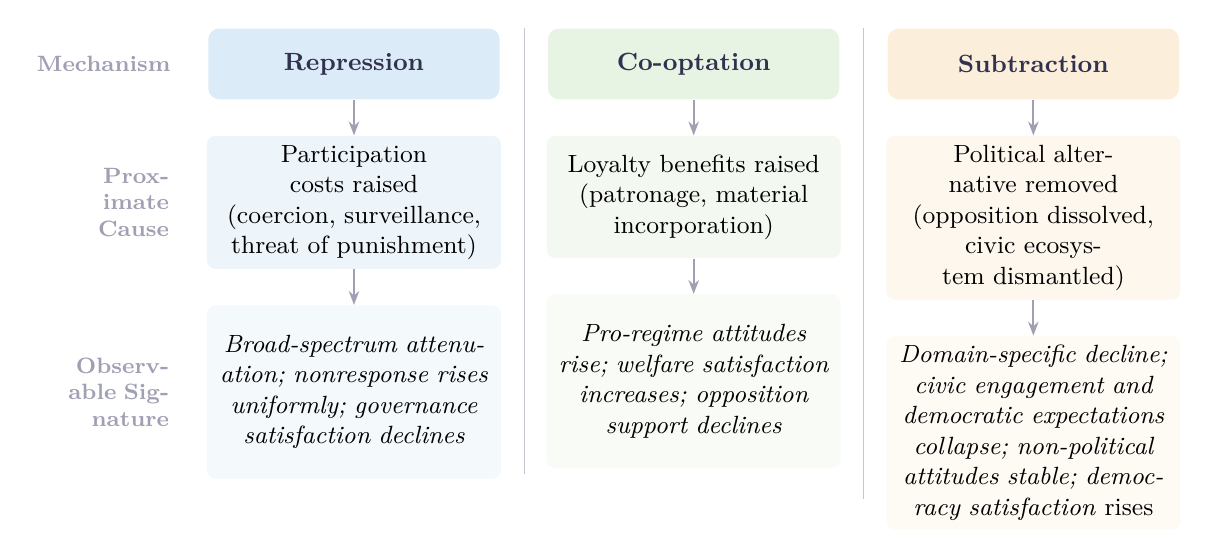
\begin{tikzpicture}[
  mech/.style  = {rectangle, rounded corners=4pt, minimum width=3.7cm,
                  minimum height=0.9cm, align=center,
                  font=\small\bfseries\color{hdrcolor}},
  cause/.style = {rectangle, rounded corners=3pt, minimum width=3.7cm,
                  minimum height=1.55cm, align=center,
                  font=\small, text width=3.5cm},
  sig/.style   = {rectangle, rounded corners=3pt, minimum width=3.7cm,
                  minimum height=2.2cm,  align=center,
                  font=\small\itshape, text width=3.5cm},
  arr/.style   = {-{Stealth[length=5pt]}, thick, color=rulecolor},
  colsep/.style= {draw=rulecolor!60, very thin},
  node distance = 0.45cm and 0.6cm
]
\node[mech,  fill=reprcolor!80] (r-mech)  {Repression};
\node[cause, fill=reprcolor!40, below=of r-mech] (r-cause)
      {Participation costs raised\\(coercion, surveillance,\\threat of punishment)};
\node[sig,   fill=reprcolor!25, below=of r-cause] (r-sig)
      {Broad-spectrum attenuation; nonresponse rises uniformly; governance satisfaction declines};

\node[mech,  fill=coopcolor!80, right=of r-mech]  (c-mech)  {Co-optation};
\node[cause, fill=coopcolor!40, below=of c-mech]  (c-cause)
      {Loyalty benefits raised\\(patronage, material\\incorporation)};
\node[sig,   fill=coopcolor!25, below=of c-cause] (c-sig)
      {Pro-regime attitudes rise; welfare satisfaction increases; opposition support declines};

\node[mech,  fill=subtcolor!80, right=of c-mech]  (s-mech)  {Subtraction};
\node[cause, fill=subtcolor!40, below=of s-mech]  (s-cause)
      {Political alternative removed\\(opposition dissolved,\\civic ecosystem dismantled)};
\node[sig,   fill=subtcolor!25, below=of s-cause] (s-sig)
      {Domain-specific decline; civic engagement and democratic expectations collapse; non-political attitudes stable; democracy satisfaction \emph{rises}};

\foreach \top/\bot in {r-mech/r-cause, r-cause/r-sig,
                        c-mech/c-cause, c-cause/c-sig,
                        s-mech/s-cause, s-cause/s-sig}{
  \draw[arr] (\top.south) -- (\bot.north);
}

\node[font=\footnotesize\bfseries\color{rulecolor}, left=0.35cm of r-mech,
      rotate=0, anchor=east, align=right] {\textsc{Mechanism}};
\node[font=\footnotesize\bfseries\color{rulecolor}, left=0.35cm of r-cause,
      rotate=0, anchor=east, align=right, text width=1.5cm] {\textsc{Proximate} \textsc{Cause}};
\node[font=\footnotesize\bfseries\color{rulecolor}, left=0.35cm of r-sig,
      rotate=0, anchor=east, align=right, text width=1.5cm] {\textsc{Observable} \textsc{Signature}};

\begin{scope}[on background layer]
  \draw[colsep]
    ($(r-mech.north east)!0.5!(c-mech.north west)$)
    -- ($(r-sig.south east)!0.5!(c-sig.south west)$);
  \draw[colsep]
    ($(c-mech.north east)!0.5!(s-mech.north west)$)
    -- ($(c-sig.south east)!0.5!(s-sig.south west)$);
\end{scope}
\end{tikzpicture}%
}% end resizebox
\caption{\textbf{Three mechanisms of political demobilization: causal pathways and observable implications.}
The subtraction mechanism is distinguished from repression and co-optation by the locus of regime action
(the political field rather than the citizenry directly) and by a domain-specific rather than broad-spectrum
observable signature. The Cambodian data are consistent with the subtraction column and inconsistent with the
repression and co-optation columns on both the placebo battery and the democracy satisfaction trajectory.}
\label{fig:mechanisms}
\end{figure}

\section{Data, Measures, and
Comparability}\label{data-measures-and-comparability}

This article draws on the Asian Barometer Survey {[}ABS; Asian Barometer
Survey (2023){]}\footnote{Data analyzed in this article were collected
  by the Asian Barometer Project (2005--2008, 2010--2012, 2013--2016,
  2020--2022), co-directed by Professors Fu Hu, Yun-han Chu, and Min-hua
  Huang, with major funding support from Taiwan's Ministry of Education,
  the National Science and Technology Council, Academia Sinica, and
  National Taiwan University. The Asian Barometer Project Office
  (www.asianbarometer.org) is solely responsible for data distribution.
  The views expressed herein are the author's own. Cambodia has been
  included in four of the six completed waves: Wave 2 (fielded 2008, N =
  1,000), Wave 3 (2012, N = 1,200), Wave 4 (2015, N = 1,200), and Wave 6
  (2021, N = 1,242). Cambodia was not included in Wave 1 (2001--2003) or
  Wave 5 (2018--2019); the latter omission is particularly
  consequential, as it means no ABS data exist from the immediate
  aftermath of the CNRP dissolution and the 2018 one-party election. The
  survey's Wave 5 fieldwork period coincided with the immediate
  aftermath of the forced dissolution of the CNRP in November 2017 and
  the July 2018 national election in which the CPP ran virtually
  unopposed---conditions under which credible public opinion research
  could not be conducted. The absence of Wave 5 is thus not an artifact
  of research design but a reflection of the political closure this
  study documents: the very phenomenon under investigation rendered
  standard survey fieldwork untenable. This gap means the analysis
  cannot observe the immediate post-dissolution period directly, a
  limitation addressed below through adjudication tests designed to
  distinguish between an acute fear response and the longer-term
  normalization pattern proposed here. The four available waves
  nevertheless bracket the critical political sequence: pre-mobilization
  (2008), peak mobilization (2012), post-crackdown selective retreat
  (2015), and post-dissolution normalization (2021).} a repeated
cross-sectional survey program administered across East and Southeast
Asia since 2001.

\begin{figure}[!htbp]
\centering
\resizebox{\linewidth}{!}{%
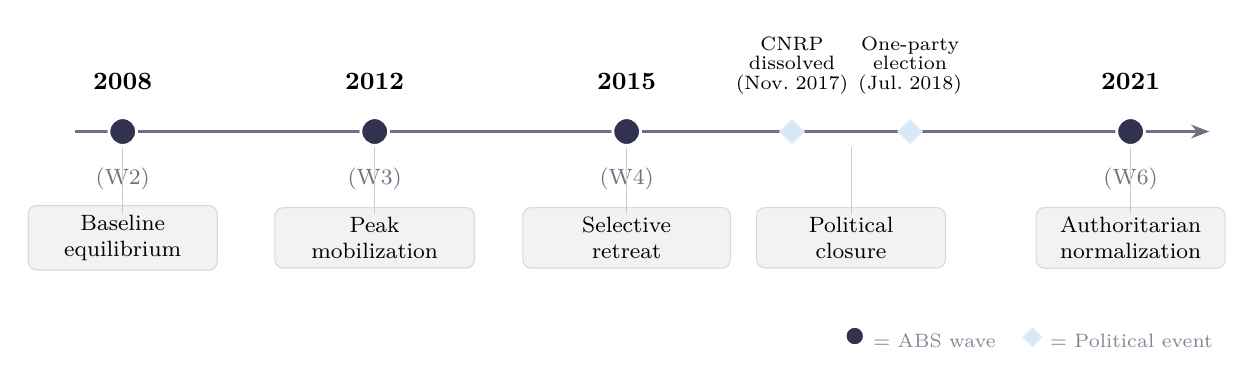
\begin{tikzpicture}[
  wave/.style   = {circle, fill=hdrcolor, draw=white, line width=1pt,
                   minimum size=10pt, inner sep=0pt},
  event/.style  = {diamond, fill=reprcolor!90, draw=reprcolor!60,
                   minimum size=9pt, inner sep=0pt},
  phase/.style  = {rectangle, rounded corners=3pt,
                   fill=gray!10, draw=gray!30,
                   minimum width=2.4cm, minimum height=0.7cm,
                   align=center, font=\footnotesize},
  ann/.style    = {font=\scriptsize, align=center, text width=2.1cm},
  node distance = 0pt
]
\draw[thick, ->, >=Stealth, color=hdrcolor!70]
  (-0.6,0) -- (13.8,0);

\def\Wa{0}
\def\Wb{3.2}
\def\Wc{6.4}
\def\Ediss{8.5}
\def\Eelec{10.0}
\def\Wd{12.8}

\foreach \x/\yr/\lbl in {
    \Wa/2008/W2,
    \Wb/2012/W3,
    \Wc/2015/W4,
    \Wd/2021/W6}{
  \node[wave] (w\yr) at (\x,0) {};
  \node[font=\small\bfseries, above=6pt of w\yr] {\yr};
  \node[font=\footnotesize\color{hdrcolor!70}, below=4pt of w\yr]
        {(\lbl)};
}

\node[event] (ediss) at (\Ediss, 0) {};
\node[event] (eelec) at (\Eelec, 0) {};

\node[ann, above=10pt] at (\Ediss, 0)
      {CNRP\\[-1pt]dissolved\\[-1pt](Nov.\ 2017)};
\node[ann, above=10pt] at (\Eelec, 0)
      {One-party\\[-1pt]election\\[-1pt](Jul.\ 2018)};

\node[phase, text width=2.0cm] at (\Wa, -1.35) {Baseline\\equilibrium};
\node[phase, text width=2.3cm] at (\Wb, -1.35) {Peak\\mobilization};
\node[phase, text width=2.4cm] at (\Wc, -1.35) {Selective\\retreat};
\node[phase, text width=1.55cm] at ({(\Ediss+\Eelec)/2}, -1.35) {Political\\closure};
\node[phase, text width=2.1cm] at (\Wd, -1.35) {Authoritarian\\normalization};

\foreach \x in {\Wa,\Wb,\Wc,\Wd}{
  \draw[gray!40, very thin] (\x,-0.2) -- (\x,-1.05);
}
\draw[gray!40, very thin]
  ({(\Ediss+\Eelec)/2},-0.2) -- ({(\Ediss+\Eelec)/2},-1.05);

\node[font=\scriptsize, color=hdrcolor!60] at (11.5, -2.6)
      {\tikz\node[wave,minimum size=7pt]{};\ = ABS wave \quad
       \tikz\node[event,minimum size=7pt]{};\ = Political event};
\end{tikzpicture}%
}% end resizebox
\caption{\textbf{The political sequence, 2008--2021.}
Filled circles mark Asian Barometer Survey waves; diamonds mark key political events.
The analysis is organised around four phases defined by the relationship between the
Cambodia National Rescue Party and the political field: pre-mobilization baseline (2008),
peak mobilization (2012), selective retreat (2015), and post-dissolution normalization (2021).
The six-year gap between Wave 4 and Wave 6 encompasses the critical closure sequence.}
\label{fig:timeline}
\end{figure}

The ABS employs face-to-face interviews with nationally representative
probability samples; response rates across the four Cambodian waves
range from approximately 80 to 90 percent.\footnote{Cambodian samples
  are stratified by province and urban/rural classification, with
  primary sampling units selected proportional to population size and
  households via random walk procedures within enumeration areas. The
  survey instrument is administered in Khmer. No post-stratification
  weights are applied; samples are treated as self-weighting, following
  ABS standard practice for single-country analyses. On ABS methodology
  and sampling design generally, see Chu et al. (2008); country-level
  details are in the ABS Technical Report for each wave.}

\subsection{Supplementary Data---The 2017 Cambodia Socio-Economic
Survey}\label{supplementary-datathe-2017-cambodia-socio-economic-survey}

The ABS data are supplemented by a single cross-section from the
Cambodia Socio-Economic Survey (SES), a nationally representative
household survey administered by the National Institute of Statistics.
The SES wave employed here (deposited with the World Bank Microdata
Library as KHM\_2018\_SAIE\_v01; N = 3,363) was collected through
face-to-face interviews with an inferred fieldwork period of
early-to-mid 2017, placing the survey in the final months before the
intensification of political closure.\footnote{The fieldwork period is
  inferred from internal temporal references: the questionnaire
  references the 2016--17 school year as current, the 2016 commune
  budget as the most recently completed fiscal cycle, and ``additional
  money paid to officials in 2016'' as a retrospective question about
  the immediately preceding year. This places collection after the
  collapse of the Culture of Dialogue but before Kem Sokha's arrest in
  September 2017 and the CNRP dissolution in November 2017.}

Six governance items from the SES are relevant to the present analysis:
perceived responsiveness of commune councillors and village chiefs
(binary agree/disagree), perceived freedom of speech and freedom of
association at the commune level (binary), perceived freedom to vote for
any party without fear (binary), and reported payment of ``tea
money''---the Cambodian vernacular for petty bribery---to government
officials in 2016 (binary). These items are not directly comparable to
the ABS instruments in scale or sampling design, and are not treated as
equivalent measures. Their value is triangulative: they establish the
state of perceived civic freedom and corruption exposure in the
immediate pre-dissolution period, a window the ABS does not cover. The
SES data are reported in Appendix D.

Detailed SES governance modules were not publicly available for the
2018--2020 fieldwork period; a phone-based COVID-focused survey
conducted in 2020 carried no political orientation or corruption items.
The absence of detailed governance survey data during the years
immediately following the CNRP dissolution is consistent with the
broader pattern of political closure documented in this article.

The analysis tracks five thematic domains across waves. For each domain,
the specific indicators, scale constructions, and cross-wave
comparability considerations are as follows.

\emph{Political participation.} Six participation items are tracked as
gate proportions---the share of the full sample reporting ever having
engaged in each activity. Of these, contacting influential persons and
attending demonstrations employ consistent wording across all four waves
and are treated as fully comparable; cross-wave comparability for other
items is documented in the appendix (Table A1).\footnote{The ABS
  participation battery employs a two-part structure: a gate question
  (``Have you ever done X?'') asked of all respondents, followed by a
  frequency question asked only of those who answer affirmatively. This
  article reports gate proportions rather than frequency means, which
  are conditional on participation and based on much smaller subsamples.
  The elected official and civil servant contact items use a narrower,
  problem-motivated framing in Wave 3 (``to complain about or seek help
  with a problem'') that differs from the broader framing in Waves 2, 4,
  and 6; cross-wave comparisons involving Wave 3 for these items are
  flagged accordingly. Petitions, demonstrations, and media contact were
  not fielded in Wave 2.} Community leader contact frequency (1--5
scale) and self-reported voter turnout (binary) supplement the gate
items.

\emph{Authoritarian governance preferences.} Four items assess
respondent evaluations of non-democratic governance alternatives:
single-party rule, strongman rule, military rule, and expert rule. Each
is measured on a consistent 1--4 scale (1 = ``very bad,'' 4 = ``very
good'') across all waves in which the item appears. Expert rule was not
fielded in Wave 2. These items are among the most stable in the ABS
instrument, with identical wording and response options across waves.

\subsection{Democratic Orientations}\label{democratic-orientations}

The analysis tracks four analytically separable dimensions of democratic
attitudes, following the growing recognition that ``democratic support''
is not a unitary construct (Bratton et al. 2004; Mattes and Bratton
2007): abstract commitment (forced-choice democracy preference and an
agree/disagree evaluative item), practical prioritization (a
democracy-vs-equality trade-off), satisfaction with how democracy works
(1--4 scale, identical wording all four waves), and feasibility
expectations (0--10 past/present/future ratings, Waves 3, 4, and 6
only).\footnote{\emph{Commitment item 1} (all four waves): forced choice
  among ``democracy is always preferable,'' ``authoritarian government
  can sometimes be preferable,'' and ``it doesn't matter'' (coded 1--3).
  \emph{Commitment item 2} (Waves 3--6): ``democracy may have its
  problems but it is still the best form of government'' (1--4
  agree/disagree; nonresponse under 2 percent in Waves 3--4, rising to
  10--13 percent in Wave 6). \emph{Prioritization} (Waves 3, 4, 6):
  five-point trade-off between political freedom and economic equality;
  a second trade-off pitting democracy against economic development is
  available all four waves but is empirically less dynamic and reported
  in Appendix Table A10. \emph{Corruption}: witnessed corruption is a
  binary indicator; Wave 2 wording is narrower than Waves 3--6 and
  treated with caution. Perceived national and local government
  corruption on consistent 1--4 scales. \emph{Media and interest}:
  political interest, news following, and political discussion on
  consistent 1--4 or 1--3 scales; internet news harmonized to a 1--6
  frequency scale across waves with differing original response
  categories.} The expectations items carry the highest nonresponse---63
percent on democratic future in Wave 6---and are treated as supporting
evidence for patterns established more robustly on the commitment,
prioritization, and satisfaction measures. The nonresponse rate is
itself analytically informative and is addressed in the alternative
mechanisms section.

Table~\ref{tbl-comparability} summarizes the comparability status of the
headline indicators.

\begin{table}

\caption{\label{tbl-comparability}Cross-Wave Comparability of Headline
Indicators}

\centering{

\centering\begingroup\fontsize{9}{11}\selectfont

\resizebox{\linewidth}{!}{
\begin{threeparttable}
\begin{tabular}[t]{>{\raggedright\arraybackslash}p{5.5cm}>{\raggedright\arraybackslash}p{1.5cm}>{\raggedright\arraybackslash}p{5.5cm}}
\toprule
Variable & Status & Notes\\
\midrule
Contacted influential person & Full & \\
Demonstration attendance & Full & \\
Single-party rule (1--4) & Full & Not fielded W2\\
Strongman rule (1--4) & Full & Not fielded W2\\
Democracy always preferable & Full & Not fielded W2\\
Democracy satisfaction (1--4) & Full & \\
Democratic future (0--10) & Full* & Not fielded W2; 63\% NR in W6\\
Democracy vs.\ equality (1--5) & Full & Not fielded W2\\
\midrule
Witnessed corruption (binary) & Partial & W2 wording narrower\\
Contacted civil servant & Partial & W3 wording differs\\
Contacted elected official & Partial & W3 wording differs\\
Internet news frequency & Partial & Scale harmonized\\
\bottomrule
\end{tabular}
\begin{tablenotes}[para]
\item \textit{Note:} 
\item Full = identical or functionally equivalent wording across all waves in which the item appears. Partial = minor wording shift or response scale change requiring caution in cross-wave comparison. Full* = wording consistent but elevated nonresponse in later waves limits inferential strength. Full detail in Appendix Table A1.
\end{tablenotes}
\end{threeparttable}}
\endgroup{}

}

\end{table}%

\emph{Analytic strategy.} The analysis is primarily descriptive:
wave-level means and proportions with 95 percent confidence intervals
(Wilson intervals for proportions; t-based for means), evaluated with
two-sample t-tests or proportion tests.\footnote{This design cannot
  establish causality in the formal sense, but can identify whether the
  timing, direction, and domain-specificity of observed shifts are
  consistent with the demobilization-by-subtraction mechanism and
  inconsistent with plausible alternatives. The analytic strategy treats
  the Cambodian sequence as a structured comparison across a documented
  political closure rather than as a natural experiment.}
Covariate-adjusted OLS models are reported in
Table~\ref{tbl-ols-controls} as a compositional robustness check,
confirming that headline patterns are not explained by demographic
differences across survey samples. The analytic leverage derives from
within-case temporal variation across a well-documented political
sequence; the alternative mechanisms section addresses causal
adjudication directly.

\begin{table}

\caption{\label{tbl-ols-controls}OLS Wave Coefficients With Demographic
Controls}

\centering{

\centering\begingroup\fontsize{9}{11}\selectfont

\resizebox{\linewidth}{!}{
\begin{threeparttable}
\begin{tabular}[t]{>{\raggedright\arraybackslash}p{1.8cm}>{\centering\arraybackslash}p{3.5cm}>{\centering\arraybackslash}p{3.5cm}>{\centering\arraybackslash}p{3.5cm}}
\toprule
 & Dem.\ future (0--10) & Dem.\ satisfaction (1--4) & Dem.\ preference (binary)\\
\midrule
Wave 4 & -1.858 (0.120)*** & -0.264 (0.031)*** & 0.131 (0.021)***\\
Wave 6 & -2.887 (0.128)*** & 0.137 (0.031)*** & 0.046 (0.022)*\\
Wave 3 & NA & 0.009 (0.031) & -0.043 (0.021)*\\
\bottomrule
\end{tabular}
\begin{tablenotes}[para]
\item \textit{Note:} 
\item OLS regression. All models include age, gender, education, and urbanicity as controls. Reference wave: W3 for democratic future; W2 for satisfaction and preference. Cell format: coefficient (SE). * $p < .05$; ** $p < .01$; *** $p < .001$. Full models with freedom-perception controls and attenuation estimates in Appendix Table A6.
\end{tablenotes}
\end{threeparttable}}
\endgroup{}

}

\end{table}%

\section{The Quiet Kingdom: Cambodia in
2008}\label{the-quiet-kingdom-cambodia-in-2008}

The first act of this story is a silence, and it is important to
understand what kind of silence it was.\footnote{Unless otherwise noted,
  the political chronology and electoral data in this section draw on
  Hughes (2010); Strangio (2014); Un (2013a); and Un (2013b)}

By 2008, Cambodia had been under continuous CPP rule for over two
decades. The party had consolidated its dominance through a patronage
network linking the central state to village-level administration, an
integrated security apparatus, a compliant judiciary, and GDP growth
averaging about 7 percent annually---the material foundation for the
regime's implicit bargain of stability in exchange for political
acquiescence (Blake 2019; Morgenbesser 2016; World Bank 2026). The
opposition was fragmented: the Sam Rainsy Party commanded a loyal but
limited urban constituency; the Human Rights Party, led by Kem Sokha,
lacked the organizational reach to threaten CPP hegemony. Neither posed
a credible challenge in isolation---a structural condition that would
change dramatically with their merger four years later (Norén-Nilsson
2015).

The Wave 2 Asian Barometer data from this period paint a portrait of a
population that was neither enthusiastic nor resistant, but simply
quiet.\footnote{Unless otherwise noted, the following scale conventions
  apply throughout: gate participation items are reported as the
  percentage of respondents who ever engaged in each activity (binary:
  ever vs.~never); community leader contact is reported as a mean on a
  1--5 scale (1 = never, 5 = often); authoritarian governance
  preferences on a 1--4 scale (1 = very bad, 4 = very good); democratic
  assessments on a 1--10 scale; corruption perceptions on a 1--4 scale
  (1 = hardly anyone, 4 = almost everyone); and media and political
  interest items on a 1--4 scale (1 = none, 4 = a great deal). Internet
  news frequency is harmonized to a 1--6 scale (1 = never, 6 = daily or
  more) across waves with differing original response categories; see
  the dedicated footnote in the Wave 3 discussion for details. Witnessed
  corruption is reported as a binary proportion. Voter turnout is
  self-reported and expressed as a percentage.} Political participation
was present but low in intensity: 43 percent of respondents reported
ever having contacted a person of influence, yet community leader
contact averaged just 1.53 on a five-point frequency scale.\footnote{Direct
  contact with elected officials and civil servants uses a
  broadly-worded `at any level' framing in Wave 2 that differs from the
  narrower, problem-motivated framing in Wave 3 and from the Wave 4 and
  6 formulations; these items are not used for cross-wave comparisons
  involving Wave 2 but are reported in the four-wave tables with
  appropriate documentation.}

\begin{table}

\caption{\label{tbl-wave2}Wave 2 (2008) Baseline: Political Orientations in Cambodia}

\centering{

\centering


\small
\renewcommand{\arraystretch}{1.15}
\resizebox{\linewidth}{!}{
\begin{tabular}{@{}lr@{\hskip 2em}lr@{}}
\toprule
\textbf{Variable} & \textbf{W2 (2008)} & \textbf{Variable} & \textbf{W2 (2008)} \\
\midrule
\multicolumn{2}{@{}l}{\textit{Political Participation}} & \multicolumn{2}{l}{\textit{Democratic Orientations}} \\[2pt]
Contacted elected official & 32.6\% (29.7--35.6) & Democratic present (0--10) & 6.72 (6.47--6.96) \\
Contacted civil servant & 31.8\% (29.0--34.8) & Democratic future (0--10) &---\\
Contacted influential person & 43.0\% (39.9--46.2) & Democratic past (0--10) &---\\
Signed petition &---& & \\
Attended demonstration &---& \multicolumn{2}{l}{\textit{Corruption}} \\[2pt]
Contacted media &---& Witnessed corruption & 27.7\% (24.9--30.6) \\
Community leader (1--5 mean) & 1.53 (1.49--1.57) & Nat'l govt corruption (1--4) & 2.86 (2.81--2.92) \\
Voted in last election &---& Local govt corruption (1--4) & 2.56 (2.51--2.61) \\[6pt]
\multicolumn{2}{@{}l}{\textit{Authoritarian Preferences (1--4)}} & \multicolumn{2}{l}{\textit{Media \& Political Interest}} \\[2pt]
Expert rule &---& Follows political news &---\\
Single-party rule & 1.79 (1.72--1.87) & Internet news (1--6) &---\\
Strongman rule & 1.60 (1.54--1.67) & Political interest (1--4) & 2.56 (2.50--2.62) \\
Military rule & 2.19 (2.11--2.27) & Discusses politics (1--3) & 1.65 (1.61--1.69) \\
\bottomrule
\end{tabular}}

\vspace{4pt}
{\footnotesize\textit{Note:} 95\% CI in parentheses (Wilson interval for proportions; $t$-based for means).---= not fielded in Wave 2. $N = 1{,}000$.}

}

\end{table}%

The authoritarian attitude measures are telling. Single-party rule was
rated at 1.79 on a four-point scale, strongman rule at 1.6, and military
rule at 2.19---not numbers of a population that embraces
authoritarianism as an ideal, but of one that has learned to live within
it. On the forced-choice democracy preference, 61.2 percent selected
``democracy is always preferable'' while 30.5 percent chose ``it doesn't
matter''---a plurality endorsement without intensity. Cambodia in 2008
was a country in political equilibrium. No dramatic spikes, no anomalous
values, no signs of the upheaval to come. The question that the next
four years would pose, with startling force, was what would happen when
that arrangement was briefly and dramatically disrupted.

\section{The Awakening: Cambodia in
2012}\label{the-awakening-cambodia-in-2012}

Something extraordinary happened in Cambodia between 2008 and 2012, and
the Wave 3 Asian Barometer data capture its imprint with unusual
clarity.\footnote{Unless otherwise noted, the political chronology and
  electoral data in this section draw on Un (2013b); Um (2014); Strangio
  (2014); and Norén-Nilsson (2015) On the 2013 election results
  specifically, see COMFREL (The Committee for Free and Fair Elections
  in Cambodia) (2013)}

Across nearly every measure of civic engagement and political
aspiration, Cambodian respondents in 2012 registered at or near the
highest values in the dataset's history. Contact with influential
persons rose from 43 percent in 2008 to 52.6 percent. Community leader
contact averaged 1.9 on a five-point frequency scale, up from 1.53. The
political activities newly tracked in Wave 3---attending demonstrations
(2.6 percent ever) and signing petitions (10.5 percent ever)---debuted
at levels consistent with a population in active political motion.

The catalyst was the formation of the Cambodia National Rescue Party in
2012, a merger of the Sam Rainsy Party and the Human Rights Party. The
CNRP unified the fragmented non-CPP political space into a single,
credible alternative with a coherent message of democratic reform,
anti-corruption, and economic justice, drawing its energy from an urban
youth demographic---the first generation born after the Khmer Rouge,
connected to the wider world through social media, and impatient with
the political settlement their parents had accepted. The July 2013
national election became the most competitive in Cambodia's post-UNTAC
history. The CNRP won 55 of 123 National Assembly seats; allegations of
electoral fraud triggered months of mass protest. For observers and
participants alike, the political settlement that had governed Cambodia
since the late 1990s appeared to be unraveling (Strangio 2014;
Morgenbesser 2017; Norén-Nilsson 2021).

The democratic expectations data tell the same story from a different
angle. Cambodian respondents in 2012 produced a mean of 9.58 on the
ten-point democratic future scale---near-universal optimism, suggesting
a population that had collectively decided democratic change was not
merely desirable but imminent. The past-present-future structure (low
past: 3.97; middling present: 5.85; exceptionally high future: 9.58) is
not the signature of a population evaluating its institutions on the
basis of lived experience---it is a hope-driven orientation, grounded in
expectation rather than experience, and therefore extraordinarily
sensitive to political events. The 2012 moment was not a peak of
abstract democratic commitment: the forced-choice democracy preference
(56.9 percent choosing ``always preferable'') actually ran \emph{lower}
than in 2008. It was a peak of democratic \emph{expectation} and
\emph{prioritization}. Nearly half of respondents (47.1 percent)
prioritized political freedom over economic equality---a level that
would not be observed again. Witnessed corruption, at 49 percent,
reflected not an increase in actual corruption but a population more
willing to name it, emboldened by opposition messaging and expanded
civic space. Political interest (2.57) and news following (3.07) stood
at the highest values in the Cambodian series.\footnote{Traditional
  values measures also peaked in Wave 3---an unexpected finding given
  that the broader mobilization was associated with youth activism. One
  possibility is that the CNRP's messaging, which blended democratic
  aspiration with Khmer cultural conservatism, activated traditional
  values alongside democratic ones; another is a general intensification
  of expressed attitudes in the charged political environment of 2012.}\footnote{The
  ABS internet news item underwent substantial scale changes across
  waves (6-point in W2/W3, 8-point in W4, 9-point in W6) and has been
  harmonized to a common 1--6 frequency scale (1 = never, 6 = daily or
  more).}

The 2012 data capture the approximate moment at which a population
collectively updated its beliefs about what was politically possible,
right before the regime demonstrated, with devastating effectiveness,
that those beliefs were wrong.

\section{The Reckoning: Cambodia in
2015}\label{the-reckoning-cambodia-in-2015}

The 2013 election confirmed the CNRP's mobilization power---55 seats to
the CPP's 68, the narrowest margin in Cambodia's modern history---but
the structural ceiling held.\footnote{Unless otherwise noted, the
  political chronology in this section draws on Chheang (2015);
  Morgenbesser (2017); and Norén-Nilsson (2019)} Fraud allegations
triggered mass protest; a January 2014 crackdown and subsequent
compromise coaxed the CNRP into parliament under a fragile ``Culture of
Dialogue'' that was less a genuine opening than a controlled
decompression: the CPP retained the security forces, the judiciary, and
the National Election Committee while progressively constraining the
CNRP through legal harassment and restrictions on assembly (Morgenbesser
2017; Norén-Nilsson 2019). By 2015 the dialogue had stalled, and the
Wave 4 survey entered the field in an atmosphere that had shifted from
the hopeful energy of 2013 to something more wary.

The Wave 4 data capture a population no longer at the peak of
mobilization but not yet in the trough of withdrawal. Contact with
influential persons held essentially steady at 55.9 percent (the
3.3-point increase from Wave 3 is not statistically significant;
\emph{p} = 0.11), and demonstration attendance, petition-signing, and
civil servant contact all edged slightly upward. The ``selective
retreat'' of 2015 is not written primarily in the behavioral data. It is
written in the attitudinal record (see Figure~\ref{fig-behavioral};
Figure~\ref{fig-attitudinal}).

\begin{table}

\caption{\label{tbl-wave3to4}Selective Retreat, 2012--2015: Wave 3 to Wave 4 Comparison}

\centering{

\centering


\small
\renewcommand{\arraystretch}{1.15}
\resizebox{\linewidth}{!}{
\begin{tabular}{@{}lrrr@{\hskip 1.5em}lrrr@{}}
\toprule
\textbf{Variable} & \textbf{W3} & \textbf{W4} & \textbf{$\Delta$} & \textbf{Variable} & \textbf{W3} & \textbf{W4} & \textbf{$\Delta$} \\
\midrule
\multicolumn{4}{@{}l}{\textit{Political Participation}} & \multicolumn{4}{l}{\textit{Democratic Expectations (0--10)}} \\[2pt]
Contacted elected off. & 4.1\% & 4.5\% & +0.4 & Dem.\ future & 9.58 & 7.72 & $-$1.86 \\
Contacted civil servant & 6.6\% & 11.0\% & +4.4 & Dem.\ past & 3.97 & 3.87 & $-$0.10 \\
Contacted influential & 52.6\% & 55.9\% & +3.3 & Dem.\ present & 5.85 & 5.06 & $-$0.80 \\
Signed petition & 10.5\% & 14.5\% & +4.0 & & & & \\
Attended demonstration & 2.6\% & 4.5\% & +2.0 & \multicolumn{4}{l}{\textit{Corruption}} \\[2pt]
Contacted media & 3.2\% & 3.4\% & +0.2 & Witnessed corruption & 49.4\% & 62.8\% & +13.4 \\
Community leader (1--5) & 1.90 & 2.00 & +0.10 & Nat'l govt (1--4) & 2.67 & 2.90 & +0.23 \\
Voted in last election & 78.7\% & 83.2\% & +4.5 & Local govt (1--4) & 2.47 & 2.56 & +0.09 \\[6pt]
\multicolumn{4}{@{}l}{\textit{Authoritarian Preferences (1--4)}} & \multicolumn{4}{l}{\textit{Media \& Political Interest}} \\[2pt]
Expert rule & 1.58 & 1.66 & +0.08 & Follows pol.\ news & 3.07 & 2.86 & $-$0.21 \\
Single-party rule & 1.97 & 1.78 & $-$0.19 & Internet news (1--6) & 1.22 & 1.82 & +0.61 \\
Strongman rule & 1.73 & 1.76 & +0.03 & Political interest (1--4) & 2.57 & 2.29 & $-$0.28 \\
Military rule & 2.19 & 1.98 & $-$0.21 & Discusses politics (1--3) & 1.45 & 1.47 & +0.02 \\
\bottomrule
\end{tabular}}

\vspace{4pt}
{\footnotesize\textit{Note:} Point estimates only; 95\% CIs reported in Table~3 and Appendix. $\Delta$ = W4 $-$ W3. Participation rows report gate proportions (\%); all other rows report wave means. $\Delta$ for proportions in percentage points; for means in scale units. $N$: W3 = 1{,}200; W4 = 1{,}200.}

}

\end{table}%

Table~\ref{tbl-wave3to4} shows the W3→W4 shifts. The attitudinal retreat
is not accompanied by a corresponding rise in authoritarian
acceptance---single-party rule dipped, military rule fell, and all four
measures remained below 2.0. The 2015 demobilization was driven by
disillusionment and tactical withdrawal, not reorientation toward
authoritarian preferences.

The democratic orientation data reveal the first signs of a decoupling
that would define the Cambodian trajectory. Abstract democratic
commitment paradoxically surged: 74.9 percent selected ``democracy is
always preferable''---the highest proportion across all four waves, up
from 56.9 percent in 2012. The crackdown of 2013--2014 had made the
ideal visible and contested, and citizens chose sides. But
prioritization began its descent simultaneously: the
pro-political-freedom share of the democracy-versus-equality trade-off
contracted from 47.1 to 34.6 percent (mean: 2.91 → 2.58, \emph{p}
\textless{} 0.001). Citizens were affirming the ideal while becoming
less willing to bear its costs. Democratic future expectations fell
nearly two points (\emph{p} \textless{} 0.001); democracy satisfaction
dropped to 2.71---its lowest value---as the gap between elevated
expectations and deteriorating reality widened. That gap would close by
2021, producing the satisfaction paradox documented in
Figure~\ref{fig-paradox}.

Witnessed corruption surged to 63 percent---its dataset peak. The
post-2013 period, with its institutional jockeying and expanded CNRP
parliamentary presence, created more visible sites of corruption, not
more corruption per se. Political interest and news following registered
modest declines, the leading edge of a trend that would deepen sharply.
The 2015 wave is the hinge: democratic hope falling but not yet crashed,
behavior intact but attitudes already retreating, authoritarian
acceptance still low. Unstable equilibrium, poised between the
aspiration of 2012 and the normalization that was about to descend.

\section{The Silence: Cambodia in
2021}\label{the-silence-cambodia-in-2021}

On November 16, 2017, the Supreme Court of Cambodia dissolved the
Cambodia National Rescue Party, citing a vaguely defined conspiracy to
overthrow the government; 118 CNRP officials were banned from political
activity, and the party's seats redistributed to CPP-aligned
formations.\footnote{Unless otherwise noted, the political chronology in
  this section draws on Un and Luo (2020); Chheang (2021); and
  Morgenbesser and Pepinsky (2019)} Kem Sokha had already been arrested
in September; Sam Rainsy remained in exile. The dissolution did not
occur in isolation. Within weeks, the \emph{Cambodia Daily} was forced
to close after receiving a disputed \$6.3 million tax bill; Radio Free
Asia's Cambodian bureau was shuttered; independent radio stations were
pressured into pro-government programming; and civil society
organizations faced intensified scrutiny under the 2015 LANGO law
(Norén-Nilsson 2021; Norén-Nilsson and Eng 2020). The July 2018
election, conducted without the CNRP, produced a CPP sweep of all 125
National Assembly seats---completing the transition, in Levitsky and
Way's typology, from competitive to hegemonic authoritarianism (Levitsky
and Way 2010; Schedler 2002).

The Wave 6 data from 2021 record the consequences.

The participation data from 2021 present a more differentiated picture
than a simple collapse narrative would suggest (see
Figure~\ref{fig-behavioral}). Contact with influential persons---the
item most directly measuring independent civic engagement---fell
sharply, from 55.9 percent in 2015 to 23.3 percent (\emph{p} \textless{}
0.001), a 33 percentage-point decline that represents one of the
steepest single-item shifts in the dataset. Community leader contact
fell to a mean of 1.39 on the frequency scale, and political discussion
dropped to 1.26 on a four-point scale---a population that had largely
stopped talking about politics with one another. Demonstration
attendance held near its 2015 level at 3.3 percent.

What complicates any uniform ``participation collapse'' characterization
is that several formal channel indicators actually rose substantially by
2021: petition-signing reached 30.5 percent, civil servant contact
climbed to 37.2 percent, and media contact rose to 12.2 percent. These
increases likely reflect the rapid expansion of internet access enabling
digital petitions and online contact, combined with the transformation
of formal institutional channels into vehicles for routine patronage
interaction under a now-uncontested regime. The divergence is itself
evidence of demobilization by subtraction---but it also preserves a
degree of citizen agency within the normalization framework. In an
environment where opposition parties, independent media, and civil
society organizations have been dismantled, citizens learn which levers
still function and redirect their efforts accordingly. The result is
engagement that is simultaneously rational at the individual level and
depoliticizing at the collective level: participation through officially
sanctioned channels rises precisely as independent civic action
collapses.

\begin{table}

\caption{\label{tbl-table3}Four-Wave Trajectory of Political
Orientations in Cambodia, 2008--2021}

\centering{

\centering\begingroup\fontsize{11}{13}\selectfont

\resizebox{\linewidth}{!}{
\begin{threeparttable}
\begin{tabular}[t]{lccc>{}ccc}
\toprule
Variable & W2 (2008) & W3 (2012) & W4 (2015) & \textbf{W6 (2021)} & \Delta W3{\textrightarrow}W6 & \Delta W4{\textrightarrow}W6\\
\midrule
\addlinespace[0.3em]
\multicolumn{7}{l}{\textbf{Political Participation}}\\
\hspace{1em}Contacted elected official & 32.6\% (29.7--35.6) & 4.1\% (3.1--5.4) & 4.5\% (3.4--5.9) & \textbf{13.3\% (11.4--15.5)} & +9.2 pp & +8.8 pp\\
\hspace{1em}Contacted civil servant & 31.8\% (29.0--34.8) & 6.6\% (5.3--8.2) & 11.0\% (9.3--12.9) & \textbf{37.2\% (34.4--40.1)} & +30.6 pp & +26.2 pp\\
\hspace{1em}Contacted influential person & 43.0\% (39.9--46.2) & 52.6\% (49.7--55.5) & 55.9\% (53.1--58.7) & \textbf{23.3\% (20.9--25.9)} & -29.3 pp & -32.6 pp\\
\hspace{1em}Signed petition & --- & 10.5\% (8.9--12.4) & 14.5\% (12.6--16.6) & \textbf{30.5\% (27.9--33.4)} & +20.0 pp & +16.1 pp\\
\hspace{1em}Attended demonstration & --- & 2.6\% (1.8--3.7) & 4.5\% (3.5--5.9) & \textbf{3.3\% (2.3--4.6)} & +0.7 pp & -1.2 pp\\
\hspace{1em}Contacted media & --- & 3.2\% (2.3--4.4) & 3.4\% (2.4--4.6) & \textbf{12.2\% (10.3--14.2)} & +9.0 pp & +8.8 pp\\
\hspace{1em}Contacted community leader (mean, 1–5) & 1.53 (1.49--1.57) & 1.90 (1.85--1.96) & 2.00 (1.95--2.06) & \textbf{1.39 (1.34--1.43)} & -0.52 & -0.62\\
\hspace{1em}Voted in last election & --- & 78.7\% (76.2--80.9) & 83.2\% (80.9--85.2) & \textbf{88.1\% (86.1--89.9)} & +9.4 pp & +4.9 pp\\
\addlinespace[0.3em]
\multicolumn{7}{l}{\textbf{Authoritarian Preferences (1–4: very bad to very good)}}\\
\hspace{1em}Expert rule & — & 1.58 (1.53--1.63) & 1.66 (1.62--1.70) & \textbf{2.11 (2.06--2.16)} & +0.53 & +0.45\\
\hspace{1em}Single-party rule & 1.79 (1.72--1.87) & 1.97 (1.91--2.03) & 1.78 (1.73--1.83) & \textbf{2.21 (2.15--2.26)} & +0.24 & +0.43\\
\hspace{1em}Strongman rule & 1.60 (1.54--1.67) & 1.73 (1.67--1.78) & 1.76 (1.71--1.81) & \textbf{2.17 (2.12--2.23)} & +0.45 & +0.42\\
\hspace{1em}Military rule & 2.19 (2.11--2.27) & 2.19 (2.12--2.25) & 1.98 (1.93--2.04) & \textbf{2.21 (2.15--2.27)} & +0.02 & +0.23\\
\addlinespace[0.3em]
\multicolumn{7}{l}{\textbf{Democratic Commitment \& Satisfaction}}\\
\hspace{1em}Democracy always preferable (\%) & 61.2\% (57.8--64.4) & 56.9\% (54.0--59.7) & 74.9\% (72.4--77.4) & \textbf{66.5\% (63.6--69.3)} & +9.7 pp & NA\\
\hspace{1em}Dem. best form of govt (1--4) & \textemdash & 3.26 (3.22--3.29) & 3.15 (3.12--3.19) & \textbf{3.20 (3.16--3.23)} & -0.06 & NA\\
\hspace{1em}Democracy vs. equality (1--5) & \textemdash & 2.91 (2.83--3.00) & 2.58 (2.49--2.67) & \textbf{2.31 (2.23--2.39)} & -0.60 & NA\\
\hspace{1em}Democracy satisfaction (1--4) & 2.97 (2.92--3.01) & 2.98 (2.94--3.02) & 2.71 (2.66--2.75) & \textbf{3.10 (3.07--3.14)} & +0.12 & NA\\
\addlinespace[0.3em]
\multicolumn{7}{l}{\textbf{Democratic Expectations (0–10 scale)}}\\
\hspace{1em}Democratic future (10pt) & — & 9.58 (9.48--9.68) & 7.72 (7.48--7.96) & \textbf{6.67 (6.45--6.89)} & -2.91 & -1.05\\
\hspace{1em}Democratic past (10pt) & — & 3.97 (3.85--4.09) & 3.87 (3.75--3.98) & \textbf{4.78 (4.65--4.92)} & +0.82 & +0.92\\
\hspace{1em}Democratic present (10pt) & 6.72 (6.47--6.96) & 5.85 (5.66--6.04) & 5.06 (4.89--5.23) & \textbf{5.77 (5.62--5.92)} & -0.08 & +0.72\\
\addlinespace[0.3em]
\multicolumn{7}{l}{\textbf{Corruption}}\\
\hspace{1em}Witnessed corruption (binary) & 27.7\% (24.9--30.6) & 49.4\% (46.5--52.3) & 62.8\% (59.9--65.7) & \textbf{14.9\% (12.9--17.1)} & -34.5 pp & -47.9 pp\\
\hspace{1em}National govt corruption (1–4) & 2.86 (2.81--2.92) & 2.67 (2.62--2.72) & 2.90 (2.86--2.94) & \textbf{2.33 (2.29--2.37)} & -0.34 & -0.57\\
\hspace{1em}Local govt corruption (1–4) & 2.56 (2.51--2.61) & 2.47 (2.42--2.52) & 2.56 (2.52--2.61) & \textbf{2.36 (2.32--2.41)} & -0.11 & -0.20\\
\addlinespace[0.3em]
\multicolumn{7}{l}{\textbf{Media \& Political Interest}}\\
\hspace{1em}Follows political news & — & 3.07 (2.99--3.14) & 2.86 (2.78--2.94) & \textbf{2.04 (1.97--2.11)} & -1.03 & -0.82\\
\hspace{1em}Internet news (1–6) & — & 1.22 (1.16--1.27) & 1.82 (1.72--1.92) & \textbf{4.66 (4.54--4.78)} & +3.45 & +2.84\\
\hspace{1em}Political interest & 2.56 (2.50--2.62) & 2.57 (2.52--2.62) & 2.29 (2.24--2.34) & \textbf{2.06 (2.01--2.11)} & -0.51 & -0.23\\
\hspace{1em}Discusses politics & 1.65 (1.61--1.69) & 1.45 (1.42--1.49) & 1.47 (1.44--1.50) & \textbf{1.26 (1.23--1.28)} & -0.20 & -0.21\\
\bottomrule
\end{tabular}
\begin{tablenotes}[para]
\item \textit{Note:} 
\item N per wave: W2 = 1,000; W3 = 1,200; W4 = 1,200; W6 = 1,242. Rows 1--6 (Political Participation) report the percentage of respondents who ever engaged in each activity (gate proportion), with 95\% CI (Wilson interval) in parentheses; $\Delta$ for these rows is in percentage points. Democracy always preferable reports the percentage selecting `democracy is always preferable' (Wilson CI). Remaining rows report unweighted wave means with 95\% CI (t-based) in parentheses; $\Delta$ is the arithmetic difference. `---' or `textemdash' indicates variable not fielded in that wave. $\Delta$ W3$\rightarrow$W6 = peak-to-trough change (W6 minus W3). $\Delta$ W4$\rightarrow$W6 = post-dissolution change (W6 minus W4). W6 column in bold marks the endpoint of the trajectory. Voted last election and corruption witnessed are binary proportions.
\end{tablenotes}
\end{threeparttable}}
\endgroup{}

}

\end{table}%

\newpage

\begin{figure}[!htbp]

\centering{

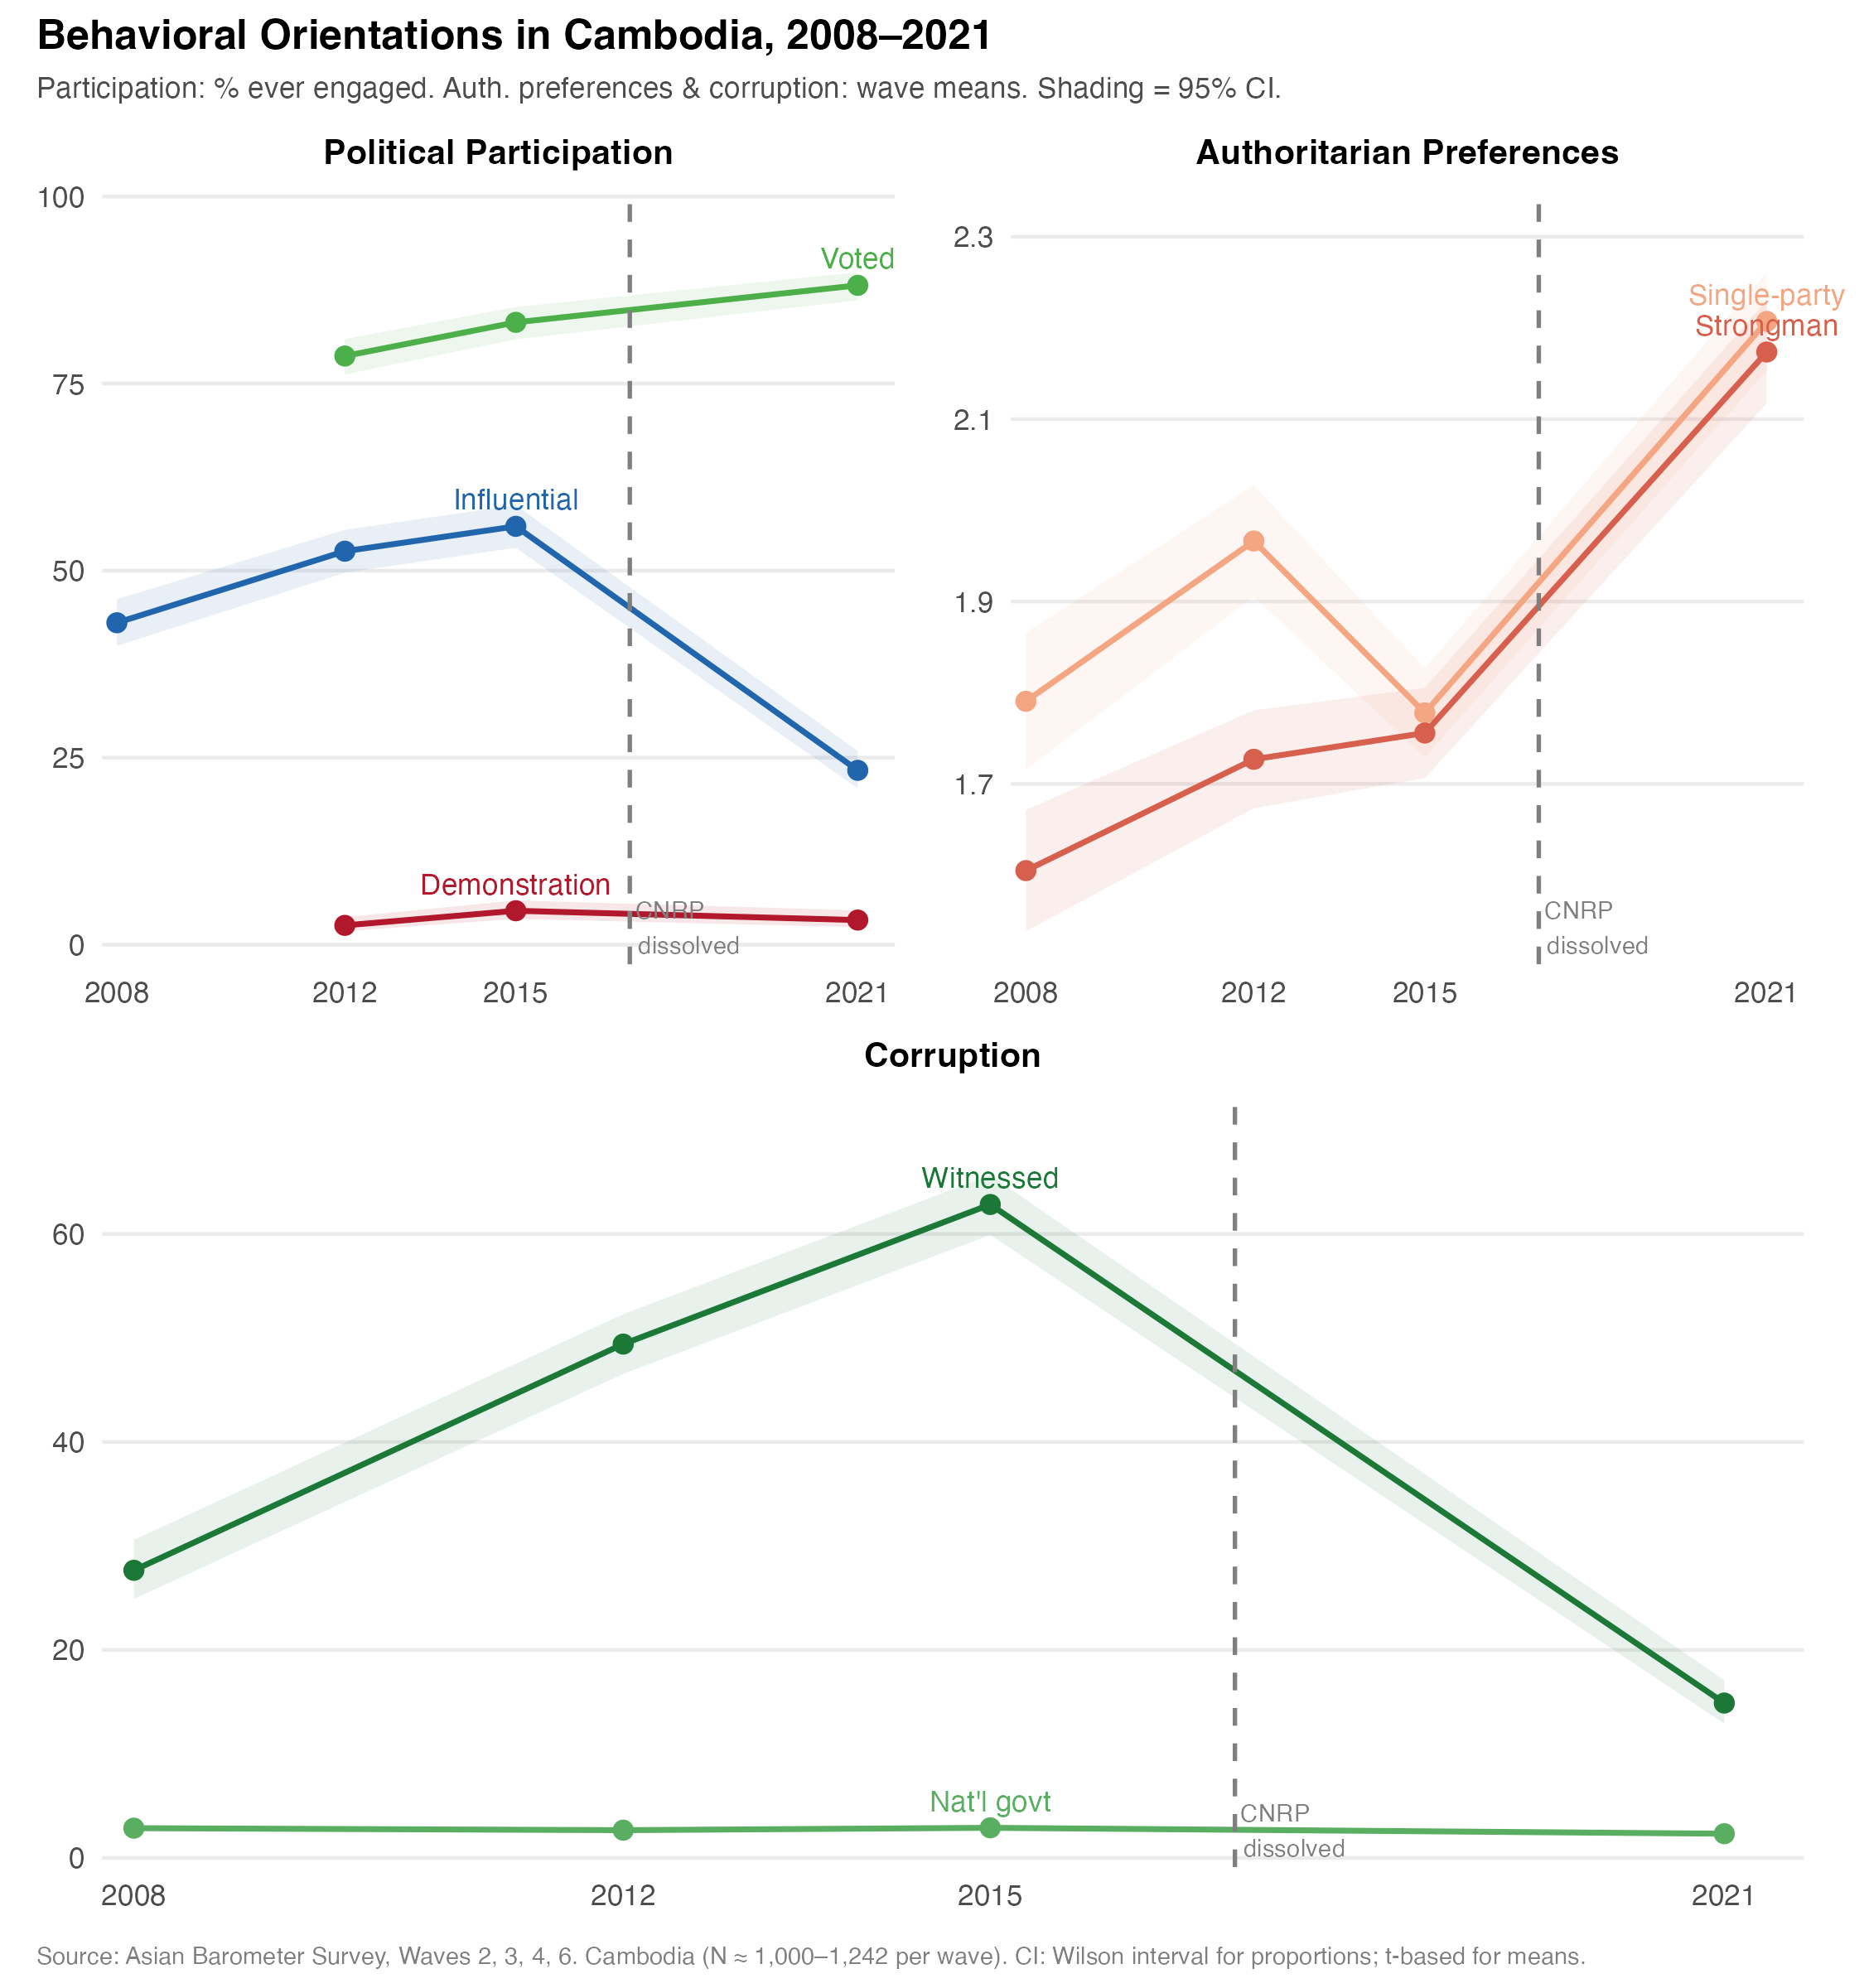
\includegraphics[width=1\linewidth,height=\textheight,keepaspectratio]{../analysis/figures/fig_behavioral.png}

}

\caption{\label{fig-behavioral}Behavioral Orientations in Cambodia,
2008--2021. Point estimates with 95\% confidence intervals (Wilson
intervals for proportions; t-based for means). Dashed vertical line
marks the 2017 CNRP dissolution. Participation panel reports gate
proportions (\% ever engaged); authoritarian preferences and corruption
panels report wave means on original scales. Source: Asian Barometer
Survey, Waves 2, 3, 4, 6.}

\end{figure}%

\begin{figure}[!htbp]

\centering{

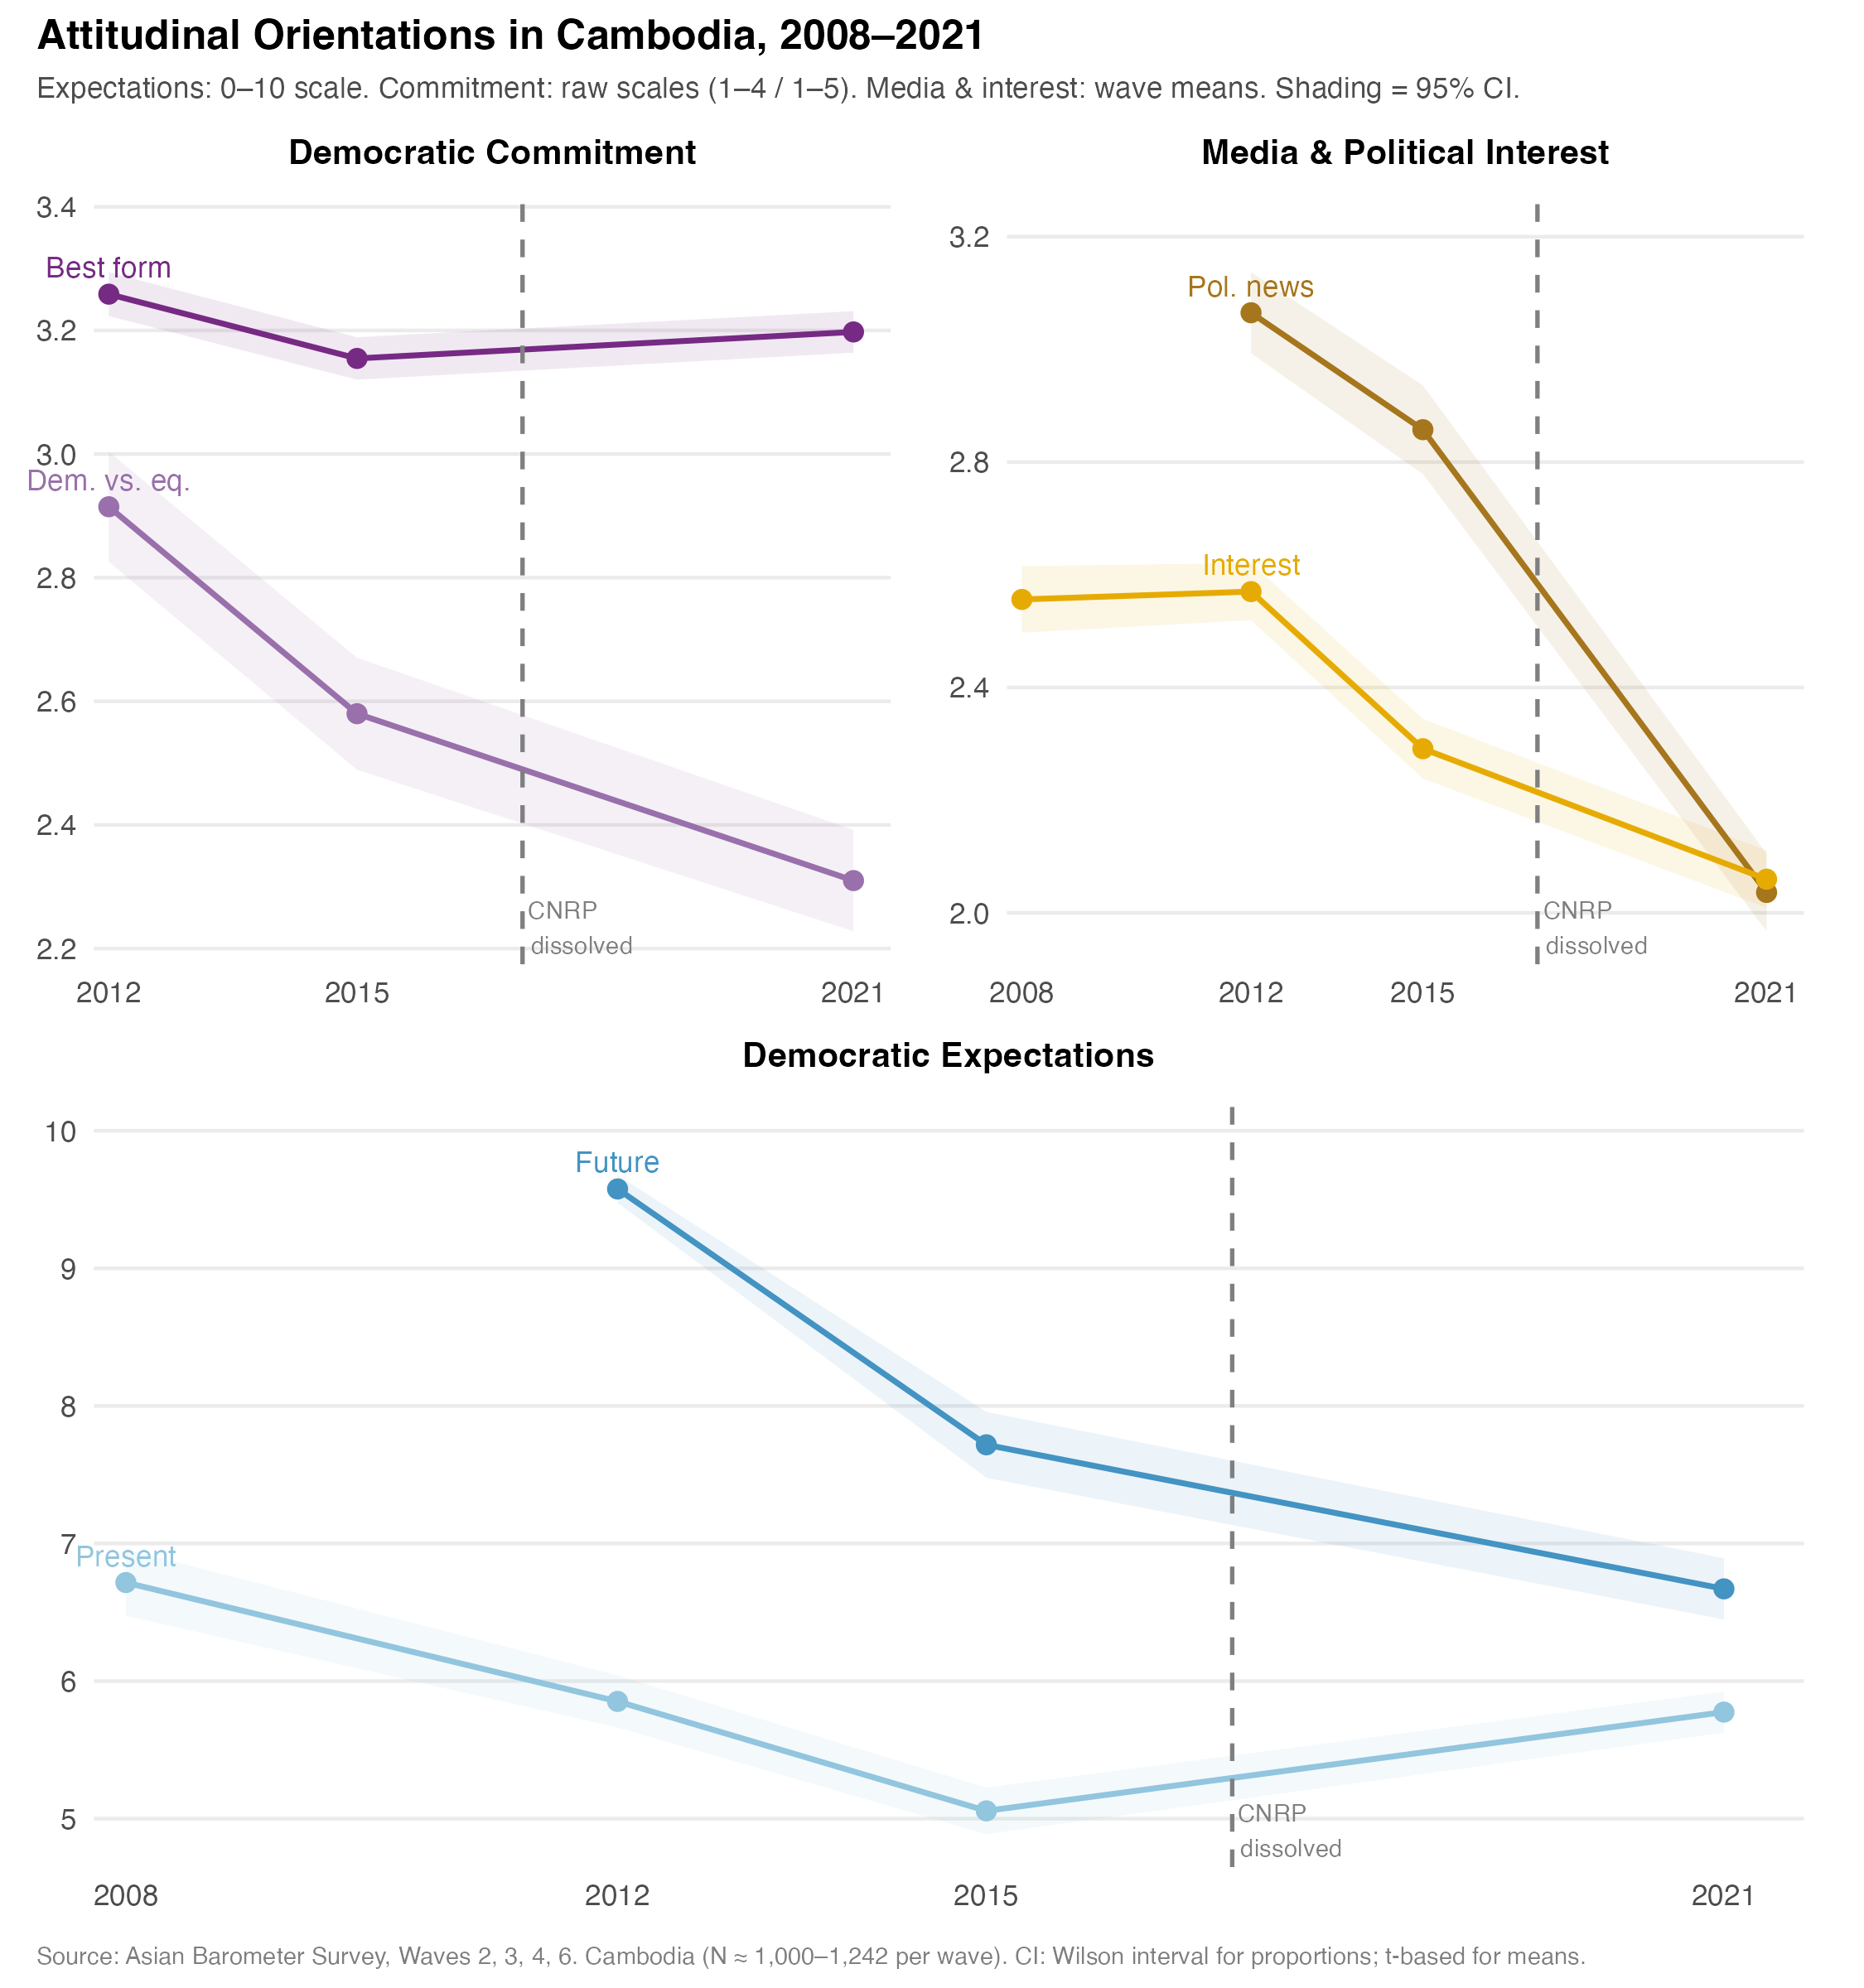
\includegraphics[width=1\linewidth,height=\textheight,keepaspectratio]{../analysis/figures/fig_attitudinal.png}

}

\caption{\label{fig-attitudinal}Attitudinal Orientations in Cambodia,
2008--2021. Point estimates with 95\% confidence intervals (t-based for
means). Dashed vertical line marks the 2017 CNRP dissolution. Democratic
Expectations panel: 0--10 scale. Democratic Commitment panel:
dem\_best\_form (1--4 mean) and dem\_vs\_equality (1--5 mean), showing
stable abstract commitment diverging from declining expectations. Media
\& Political Interest panel: wave means on original scales. Source:
Asian Barometer Survey, Waves 2, 3, 4, 6.}

\end{figure}%

\section{Democratic Orientations in
2021}\label{democratic-orientations-in-2021}

The democratic orientation data from Wave 6 complete the divergence
pattern that first appeared in 2015, now with the full force of the
post-dissolution political closure behind it (see
Figure~\ref{fig-attitudinal}).

Abstract democratic commitment, remarkably, survived the dissolution
largely intact. ``Democracy may have its problems but it is still the
best form of government'' registered a mean of 3.20 in Wave 6---between
``agree'' and ``strongly agree,'' statistically indistinguishable from
its Wave 4 value (3.15; \emph{p} = 0.080) and only marginally below the
Wave 3 peak of 3.26 (\emph{p} = 0.014). The stability of this item
across a period in which every other democratic indicator declined
sharply is among the most important findings in the dataset. Cambodians
in 2021 continued to endorse democracy as an ideal at rates essentially
unchanged from the peak mobilization of 2012. Whatever the dissolution
accomplished, it did not produce ideological conversion.

The forced-choice democracy preference declined from its Wave 4 peak of
74.9 percent to 66.5 percent---still a clear majority. The critical
diagnostic is where the movement went: the ``doesn't matter'' category
continued to decline to 17.5 percent, its lowest level across all four
waves, while ``authoritarian government can sometimes be preferable''
more than doubled from 6.1 to 16.0 percent. This distribution is
inconsistent with generalized apathy and inconsistent with fear-driven
acquiescence; it is consistent with a specific pragmatic recalculation
by citizens who reassessed their democratic commitment in light of a
political reality in which the democratic alternative no longer existed.

Democratic prioritization reached its lowest recorded level. The
pro-political-freedom share of the democracy-versus-equality trade-off
contracted from 47.1 percent in 2012 to 21.7 percent in 2021---a
collapse of more than half. The ``both equally important'' midpoint
expanded from 2.5 to 15.1 percent, while ``authoritarian sometimes
preferable'' grew modestly. The citizens most susceptible to
deprioritization were those whose commitment to political freedom had
been moderate and conditional---the pragmatic middle that the
normalization framework predicts would be most responsive to the closure
of democratic possibility.

The democratic expectation items continued their descent, though the 63
percent nonresponse on the democratic future item and 43 percent on the
democratic present mean these estimates describe only the minority of
respondents who retained enough political engagement to formulate a
numerical judgment. Treated as supporting evidence rather than
independent findings, the democratic future rating fell from 7.72 in
2015 to 6.67 in 2021 (\emph{p} \textless{} 0.001)---a drop of nearly
three points from the extraordinary 9.58 recorded in 2012.

The most robust single finding from the Wave 6 democratic orientation
battery is the satisfaction paradox (Linde and Ekman 2003; Valgarðsson
and Devine 2022): democracy satisfaction rose to 3.10---its highest
value across all four waves, on an item with only 6.4 percent
nonresponse---in the least democratic moment in the country's modern
history. Figure~\ref{fig-paradox} shows why. Satisfaction is a function
of the gap between expectations and perceived reality; by 2021 that gap
had closed from below, as expectations collapsed while the regime
delivered stability through its patronage infrastructure. The
satisfaction recovery is the clearest single indicator of adaptive
preference formation in the dataset.

\begin{figure}[!htbp]

\centering{


\includegraphics[width=0.9\linewidth,height=\textheight,keepaspectratio]{cd_manuscript_files/figure-pdf/fig-paradox-1.pdf}

}

\caption{\label{fig-paradox}\textbf{The satisfaction paradox, 2012--2021.}
Democratic future expectations (0--10 scale) and democracy satisfaction
rescaled to the same range (original 1--4 scale shown on right axis).
Shaded region marks the expectation--reality gap. The gap closes by 2021
as expectations collapse while satisfaction rises---the empirical
signature of authoritarian normalization. Dashed vertical line marks the
2017 CNRP dissolution. Source: Asian Barometer Survey, Waves 3, 4, 6.}

\end{figure}%

The authoritarian acceptance measures moved in mirror image. All four
alternative governance indicators rose to their highest levels: expert
rule to 2.11, single-party rule to 2.21, strongman rule to 2.17, and
military rule to 2.21. The jump was concentrated entirely in the
W4-to-W6 period---the six years that encompassed the CNRP's destruction
and the subsequent one-party election. What had been stable or declining
through 2015 now surged.

The authoritarian acceptance measures remain around 2.2 on a four-point
scale---below the midpoint. Cambodians are not rating authoritarianism
as ``good''; they are rating it as slightly less bad than before. The
timing---concentrated after the removal of the democratic alternative,
not during earlier repressive tightening---points toward adaptive
preference formation rather than genuine conversion. This is not a
population that has found a new political faith. It is a population that
has stopped believing the old one was achievable.

The article proposes the term authoritarian normalization to describe
this process, distinguishing it from authoritarian legitimation.
Legitimation implies that citizens have come to view the regime as
rightfully entitled to rule---on the basis of performance, ideology, or
tradition; normalization implies something weaker but potentially more
durable: citizens have adjusted their expressed preferences to align
with the only available reality. The vulnerabilities differ accordingly.
A regime sustained by legitimation is threatened when performance
falters; one sustained by normalization is threatened when alternatives
re-enter the political imagination.

The Cambodian pattern is not performative compliance in Wedeen's sense,
where citizens maintain private skepticism while publicly enacting
belief (Wedeen 1998). Survey responses are private, and the attitudinal
shifts reflect genuine reorientation: citizens moved into conditional
authoritarianism rather than noncommittal safe responses, and the shifts
cut uniformly across demographic subgroups. The
democracy-versus-equality trajectory---from near-parity in 2012 to a
two-to-one margin favoring equality by 2021---bears the hallmarks of
Elster's adaptive preference formation (Elster 2016, orig. 1983;
Przeworski 2022), but the adaptation is partial. Abstract endorsement of
democracy proved resilient while the willingness to prioritize it
collapsed. A regime that eliminates alternatives need not change what
citizens believe in principle; it need only wait for the practical
implications of those beliefs to atrophy (Jones and Cowan 2025).

The corruption data offer perhaps the most unsettling evidence of
normalization. Witnessed corruption collapsed from 63 percent in 2015 to
15 percent in 2021. Perceived national government corruption also
declined, from 2.9 to 2.33 on the four-point scale. On the surface,
these numbers might suggest genuine anti-corruption progress. The CPP
did conduct selective anti-corruption campaigns during this period,
targeting rivals and politically inconvenient officials. But the
magnitude of the witnessed-corruption decline---from nearly two-thirds
to one-seventh of the population---is too large to explain through
policy alone.

The more parsimonious explanation is that the corruption decline
reflects the same demobilization process visible in the participation
data. When citizens withdraw from political life---when they stop
contacting officials, stop attending meetings, stop engaging with
governance institutions---they also reduce their exposure to the sites
where corruption is experienced and observed. A population that does not
petition, does not demonstrate, and does not contact civil servants is
also a population that has fewer occasions to witness a bribe demanded
or a favor exchanged. Demobilization, in this reading, does not merely
reduce political action; it reduces the perceptual evidence that
political action might address. The regime becomes less corrupt not
because it has reformed but because citizens have stopped looking.

External assessments corroborate this interpretation: Cambodia's
Transparency International CPI score moved from 21 to 23 over the study
period, registering no meaningful improvement even as survey-reported
witnessing of corruption collapsed fourfold (Transparency International
2023). An alternative and not mutually exclusive explanation invokes the
survey environment itself: in a political climate where the opposition
has been criminalized, respondents may calculate that acknowledging
witnessed corruption carries risks, and the social desirability bias
literature confirms that such effects intensify under political
constraint (Schedler and Sarsfield 2007; Frye et al. 2017). The two
mechanisms---reduced exposure through demobilization and increased
reticence through social desirability pressure---likely operate in
tandem.

The voter turnout paradox completes the portrait. Self-reported voting
rose from 79 percent in 2012 to 88 percent in 2021, even as all other
forms of political engagement collapsed. The 2018 election made the
ritual character of Cambodian voting unusually visible: the
CNRP-in-exile's ``clean finger'' campaign transformed polling-station
ink from an anti-fraud measure into a tool of social surveillance, with
factory workers warned of wage deductions for returning without inked
fingers (McCargo 2018). Voting in a one-party election is not a
political act in the same sense as voting in a competitive one; it is a
demonstration of compliance. The fact that turnout rises precisely as
meaningful engagement collapses suggests that Cambodians understand the
distinction even as they perform the ritual.\footnote{The international
  orientation data add a final dimension to the normalization portrait.
  Cambodian assessments of Chinese influence in the region grew more
  positive between Waves 4 and 6, rising from 2.69 to 2.88 on a
  four-point scale measuring perceived benefit versus harm. More
  striking still, expectations of future Asian---implicitly
  Chinese---regional influence climbed from 2.74 in Wave 4 to 3.3 in
  Wave 6, a trajectory that places Cambodia among the most
  China-positive publics in the ABS dataset. This is consistent with
  Cambodia's deepening alignment with Beijing during this period,
  visible in Belt and Road infrastructure investment, the Ream Naval
  Base controversy, and Cambodia's consistent support for Chinese
  positions within ASEAN. But it also fits the normalization logic: as
  democratic futures recede and Western-aligned political alternatives
  are eliminated, alignment with the ascendant authoritarian power in
  the region becomes the natural orientation of a population adjusting
  to the available political reality. A paired comparison with Vietnam
  or the Philippines---where territorial disputes drive China
  perceptions in sharply negative directions despite similar economic
  interdependence---would sharpen this point considerably (Strangio
  2020).}

Political news following fell to 2.04, political interest to 2.06, and
political discussion to 1.26---the lowest values across all four waves.
The internet news variable throws this withdrawal into sharp relief:
harmonized consumption rose to 4.66 by Wave 6, reflecting rapid
expansion of internet infrastructure. Cambodians in 2021 had far greater
access to online information than at any previous wave, yet their
political interest and news following fell to historic lows. The
infrastructure for engagement had expanded; the will to use it for
political purposes had collapsed. Demobilization, once initiated through
the removal of the political alternative, generates its own sustaining
momentum through this informational feedback loop.

The Cambodia of 2021 is, in a sense, the inverse of the Cambodia of
2012. Where the earlier moment was characterized by activation across
all dimensions---participation, aspiration, attention, even the
willingness to name corruption---the later moment is characterized by
withdrawal across all the same dimensions. The symmetry is striking and,
for the theoretical argument, essential. It suggests that what changed
between the two moments was not any single attitude or behavior but the
underlying orientation from which attitudes and behaviors derive---what
might be called the perceived horizon of political possibility. When
that horizon expanded, everything expanded with it. When it contracted,
everything contracted.

\section{Alternative Mechanisms and
Adjudication}\label{alternative-mechanisms-and-adjudication}

The preceding narrative has interpreted the synchronized attitudinal and
behavioral shifts across ABS waves as evidence of demobilization by
subtraction. Before drawing theoretical implications, it is necessary to
adjudicate this interpretation against four competing explanations:
preference falsification under intensified repression, pandemic-era
behavioral disruption, technological channel substitution, and
generational replacement. Each generates distinct observable predictions
that can be evaluated against the available data.

\emph{Preference falsification.} The most direct challenge holds that
the observed shifts reflect increased survey reticence under harsher
post-2017 conditions rather than genuine attitude change. Item
nonresponse on democratic expectations rose substantially---from 24 to
63 percent on the democratic future item---consistent with an
environment in which some respondents feel uncomfortable evaluating
their country's democratic trajectory.\footnote{Mean nonresponse across
  all political items rose from approximately 5 percent in Wave 3 to 14
  percent in Wave 6, consistent with either increased reluctance or
  decreased political engagement.}

Three considerations limit the scope of this alternative. First, if
survey reticence were the primary driver, it should manifest
broadly---but straightlining rates on the authoritarian preferences
battery actually \emph{declined} from Wave 4 (38 percent) to Wave 6 (35
percent), and acquiescence rates remained low and stable. Second, the
demobilization pattern began before the most intensive period of
political closure: democratic future expectations fell nearly two points
between Waves 3 and 4, and political interest declined, well before the
CNRP dissolution. Third, non-political placebo items---national pride,
family economic situation, perceived economic change---show no
systematic decline across waves; generalized reticence would be expected
to suppress these as well.

The most direct empirical test draws on ABS items measuring perceived
freedom of speech and freedom to organize. Adding both as covariates in
OLS models predicting democratic future expectations, satisfaction, and
preference produces virtually no attenuation: the Wave 6 coefficient on
democratic future expectations changes by 0.4 percent. The moderation
pattern runs opposite to the preference-falsification prediction:
declines in democratic future expectations are concentrated among
respondents who perceive \emph{more} freedom of speech, not less (Wave 4
interaction: \(\beta\) = -1.88, \emph{p} \textless{} .001; Wave 6:
\(\beta\) = -1.18, \emph{p} \textless{} .001). The deepest
disillusionment runs through precisely those who feel most free to
express it---a pattern consistent with genuine preference revision
rather than strategic concealment.

The nonresponse gradient across the democratic orientation battery is
itself analytically informative. Items with the lowest nonresponse---the
forced-choice democracy preference (13.4 percent), the
democracy--equality trade-off (8.1 percent)---are those requiring
respondents to select among pre-defined positions. Items with the
highest nonresponse---democratic future (63 percent), democratic present
(42.5 percent)---require generating a numerical judgment about
Cambodia's democratic trajectory. Citizens can still answer whether
democracy is desirable in the abstract, but increasingly decline to
evaluate where their country sits on a democratic continuum. The 63
percent who did not answer the democratic future item and the 37 percent
who answered with diminished expectations are complementary expressions
of the same process.

\section{Partisan Heterogeneity and the Scope of
Demobilization}\label{partisan-heterogeneity-and-the-scope-of-demobilization}

If subtraction operates through removal of the opposition specifically,
attitudinal shifts should concentrate among former CNRP supporters, who
lost their vehicle for political expression, rather than among CPP
supporters, whose political home remained intact. The ABS vote choice
items permit a direct test.

The partisan distribution across waves is itself the first piece of
evidence. In Wave 4 (2015), CNRP voters constituted 21.3 percent of the
sample and CPP voters 50.8 percent, with 17.2 percent nonvoters and 7.2
percent declining to answer. By Wave 6 (2021), the CNRP share had
collapsed to 2.7 percent---34 respondents, a residual so small it is
analytically uninformative except as a marker of the dissolution's
completeness. The CPP share returned to 60.1 percent, absorbing an
unknown proportion of former CNRP supporters who reported voting CPP in
the uncontested 2018 election. The DK/Refuse category nearly tripled,
from 7.2 to 18.8 percent. The redistribution of the CNRP's former
constituency---into CPP voting, nonvoting, or refusal to
answer---\emph{is} the subtraction documented at the level of individual
survey responses.

The W4-to-W6 decomposition of key outcomes by partisan group yields a
finding that initially appears to cut against the subtraction-specific
mechanism: the shifts are broadly uniform. Contact with influential
persons---the clearest measure of independent civic engagement---dropped
by approximately 30 percentage points across all groups: 35.1 points
among CPP voters, 30.9 among CNRP voters, 29.9 among nonvoters, and 25.6
among those declining to answer. Democratic future expectations declined
by 1.27 to 1.39 points across groups. Single-party rule acceptance rose
by 0.29 to 0.47 points. The absence of partisan heterogeneity is robust:
no group was spared the demobilization, and no group experienced it with
distinctive severity.

Two considerations complicate the interpretation of this uniformity as
evidence against the subtraction mechanism. The first is methodological.
The W6 partisan categories are themselves \emph{products} of the
dissolution. The 746 respondents classified as ``CPP voters'' in Wave 6
include an unknown number of former CNRP sympathizers who voted CPP in a
one-party election---citizens for whom ``CPP voter'' is a
post-dissolution category imposed by the absence of alternatives rather
than a stable partisan identity. The DK/Refuse category, which tripled
to 18.8 percent, likely contains the most resistant former CNRP
supporters---those who could neither bring themselves to report voting
CPP nor risk identifying with a criminalized party. Their democratic
orientation profile in Wave 6 is consistent with this reading: they
registered the lowest proportion selecting ``democracy always
preferable'' (61.1 percent) and the highest rate of conditional
authoritarianism (18.1 percent) of any group---a pattern more consistent
with suppressed democratic preferences under duress than with genuine
authoritarian conversion. The dissolution did not merely change
attitudes; it destroyed the partisan categories through which
differential effects could be measured.

The second consideration is theoretical. The prediction that CNRP
supporters should be differentially affected assumes subtraction
operates like losing one's team. The framework advanced here operates at
a different level: the removal of the credible alternative restructures
the political field itself, not merely the partisan calculus of
opposition supporters. CPP voters in 2015 inhabited a competitive system
in which political information served a decision-making function and
contacting persons outside the party apparatus had strategic rationale;
CPP voters in 2021 inhabited a one-party state in which neither
condition obtained. The uniformity of the observed shifts is precisely
what a field-level mechanism predicts---and what a party-level mechanism
does not.

\section{Supplementary Evidence from the 2017 Socio-Economic
Survey}\label{supplementary-evidence-from-the-2017-socio-economic-survey}

The 2017 Cambodia Socio-Economic Survey provides a second-instrument
snapshot of civic orientations in the final months before the CNRP
dissolution, partially addressing the temporal gap between ABS Waves 4
(2015) and 6 (2021). The SES data are not directly comparable to the ABS
in scale or design, but the directional evidence is informative.

In early-to-mid 2017, 86.1 percent of SES respondents reported freedom
to speak without fear, 87.9 percent reported freedom to join
organizations without fear, and 94.0 percent reported freedom to vote
for any party without fear---near-universal agreement, recorded in the
final months before the elimination of the only meaningful alternative
party. The political closure that followed was not acting on a
population that already felt constrained. These figures establish the
subjective distance between the pre-dissolution civic environment and
the post-dissolution environment documented in Wave 6.

The SES tea money item corroborates the corruption trajectory from a
more behaviorally concrete instrument: 34.9 percent of respondents
reported paying additional money to officials in 2016 to get things
done. This direct bribery measure confirms that petty corruption
remained widespread in the immediate pre-dissolution period. With the
ABS witnessed-corruption item registering 63 percent in 2015 and 15
percent in 2021, the SES rate of 34.9 percent for 2016 falls precisely
between these values on a narrower measure, making it more difficult to
attribute the subsequent ABS collapse to genuine anti-corruption
progress.

Satisfaction with local governance was high: 88.2 percent agreed that
commune councillors are ``helpful and responsive at solving problems,''
and 89.4 percent agreed that the village chief ``generally works for the
benefit of citizens.'' These figures are consistent with the CPP's
patronage infrastructure functioning effectively at the commune
level---the same infrastructure into which, the article argues, citizens
redirected their engagement after the dissolution foreclosed independent
channels. The post-dissolution rise in civil servant contact (from 11
percent in Wave 4 to 37 percent in Wave 6) landed on institutional
ground that citizens already found functional.

Detailed SES governance modules were not publicly released for
2018--2020; the data gap mirrors the ABS Wave 5 absence discussed
above.\footnote{The only post-dissolution SES data publicly available
  contain a single item on satisfaction with the government's handling
  of COVID-19. The systematic unavailability of civic orientation data
  across both survey programs during the years immediately following the
  CNRP dissolution is itself consistent with the political closure
  documented here.}

\emph{Pandemic-era behavioral disruption.} Wave 6 was collected during
the COVID-19 pandemic, and public health restrictions could
independently depress physical participation measures. The concern is
legitimate but bounded. The key attitudinal shifts---the decline in
democratic future expectations, the rise in authoritarian governance
acceptance---are not plausibly explained by pandemic restrictions, which
constrain behavior but have no direct mechanism for altering governance
preferences. The decline in democratic expectations began in Wave 4
(2015), six years before the pandemic. Demonstration attendance held
essentially constant between Wave 4 and Wave 6 (4.5 to 3.3 percent),
while the sharpest participation decline occurred in contacting
influential persons, an activity requiring no face-to-face contact. The
pandemic may have amplified certain behavioral measures; it cannot
account for the pattern's breadth, direction, or temporal
onset.\footnote{One placebo item does register a notable decline:
  interpersonal trust fell from 14 percent (Wave 4) to 5 percent (Wave
  6) on the binary ``most people can be trusted'' item. This drop is
  consistent with the social atomization documented in pandemic-era
  survey research across multiple countries and may also reflect broader
  erosion of social cohesion under intensified authoritarianism (Aassve
  et al. 2021). However, the fact that this is the only non-political
  item showing a substantial decline---while national pride, family
  economic assessment, and perceived economic change all remain
  stable---suggests a localized effect rather than a general
  contamination of the survey environment.}

\emph{Temporal resolution and the dissolution-as-keystone
interpretation.} The six-year gap between Wave 4 (2015) and Wave 6
(2021) means the analysis cannot determine whether the sharpest
attitudinal changes occurred as an acute shock immediately following the
dissolution, accumulated gradually through 2021, or reflect primarily
the cumulative repressive apparatus that accompanied it. Elements of all
three models likely operated simultaneously. Two considerations favor
the subtraction-centered interpretation over the repression-centered
alternative. First, the attitudinal trajectory began before the most
intensive period of repression: democratic future expectations fell
nearly two points and political interest declined between Waves 3 and 4,
when the CNRP was under selective pressure but still functionally
intact. If cumulative repression were the primary driver, onset should
concentrate post-2017. Second, the domain-specificity of the shifts is
more consistent with a mechanism operating through the structure of
political alternatives than with generalized intimidation, which would
be expected to depress expressed attitudes across domains. The
dissolution is treated here as the keystone of the closure process---the
act that restructured the political field---even as the accompanying
repressive measures amplified and accelerated those adjustments.

The domain-specificity pattern constitutes the strongest evidence
against a fear-centered interpretation. National pride, family economic
assessment, and perceived economic change are all statistically stable
between Wave 4 and Wave 6, while large directional shifts are
concentrated in political aspiration, civic engagement, and democratic
prioritization---precisely the domain the dissolution restructured.
Generalized fear produces broad-spectrum attenuation (see
Figure~\ref{fig:mechanisms}); the Cambodian data show selectivity. Full
placebo battery results are in Appendix Table A3.

\emph{Technological channel substitution.} The finding that
participation through formal channels rose between Wave 4 and Wave
6---petition-signing, civil servant contact, and media contact all
increased---while contact with influential persons outside the state
apparatus declined, could reflect a shift in participation modalities
driven by smartphone and internet penetration rather than political
demobilization. If citizens simply migrated from informal, face-to-face
civic engagement to digitally mediated formal channels, the resulting
pattern would resemble demobilization even if total civic engagement
were unchanged or increasing.

This interpretation is difficult to sustain for two reasons. First, it
cannot explain the concurrent attitudinal shifts: channel substitution
might redistribute participation across modes but provides no mechanism
for the simultaneous decline in democratic expectations, rise in
authoritarian acceptance, and collapse of political interest. If
citizens were merely engaging through different channels, their
attitudes toward democracy and authoritarianism should remain stable.
They did not. Second, the formal channels that expanded---petitioning,
contacting civil servants, contacting media---are precisely those most
compatible with regime-managed participation under hegemonic
authoritarianism. The rise of these channels alongside the collapse of
independent engagement is more consistent with the substitution of
participatory form for participatory substance than with genuine channel
migration.

\emph{Generational replacement.} Cambodia's young population and rapid
demographic change raise the possibility that apparent attitudinal
shifts across waves reflect cohort replacement rather than
within-individual attitude change: the politically activated youth of
2012 aged into their thirties by 2021, while a new cohort with no memory
of the CNRP mobilization entered the survey frame. If the post-2017
shifts are concentrated among younger respondents, compositional change
rather than demobilization could be driving the aggregate pattern.

The subgroup decompositions do not support this interpretation. The key
shifts between Wave 4 and Wave 6 are broad-based across age groups,
education levels, and urban/rural residence. Contact with influential
persons declined among under-30s (51.5 to 22.5 percent), 30--49
year-olds (55.8 to 24.8 percent), and over-50s (59.9 to 21.5 percent)
alike. Single-party rule acceptance rose across all three age groups.
Political interest fell uniformly regardless of age, education, or
urbanicity. If generational replacement were the primary mechanism, the
shifts should concentrate in the youngest cohort or attenuate among
older respondents who experienced the CNRP period directly; instead, the
pattern is strikingly uniform. This breadth is consistent with a
population-wide reorientation rather than a compositional artifact.

Taken together, the adjudication tests support the
demobilization-by-subtraction interpretation while acknowledging that
the 2021 data likely reflect some degree of pandemic amplification and
elevated survey reticence on the most politically sensitive items. The
core finding---synchronized, domain-specific shifts in political
orientations that began before the pandemic, cut across all demographic
subgroups, and leave non-political attitudes largely untouched---is more
consistent with genuine attitudinal adjustment to political closure than
with any single alternative mechanism.

\section{Conclusion}\label{conclusion}

The mechanism identified here---the restructuring of citizen
orientations through the removal of political alternatives---operates
wherever dominant-party regimes consolidate power. Four theoretical
implications bear emphasis.

The first concerns the mechanism itself. Demobilization by subtraction
does not operate by eroding democratic values. Abstract democratic
commitment remained essentially stable across the Cambodian study
period; a clear majority of respondents in 2021 endorsed democracy as
the best form of government at rates statistically indistinguishable
from 2012. What collapsed was not the ideal but the willingness to
prioritize it against competing goods and, on the more tentatively
measured expectation items, the perceived horizon within which the ideal
could be realized. The breadth of that collapse---uniform across CPP and
former CNRP voters alike---confirms that the mechanism operates at the
level of the political field rather than the partisan calculus of
individual supporters. CPP voters did not lose their party; they lost a
political system in which independent information and
outside-the-apparatus contact served any strategic purpose. The
pro-political-freedom share contracted from 47 to 22 percent; democracy
satisfaction paradoxically rose to its highest recorded level
(Figure~\ref{fig-paradox}). The divergence between resilient ideals and
collapsing prioritization suggests that democratic attitudes in
authoritarian contexts have at least three partially independent
dimensions---ideal endorsement, practical prioritization, and
feasibility expectation---that respond to the structure of available
political alternatives in characteristically different ways (Jones and
Cowan 2025). Cross-national surveys that aggregate these dimensions into
a single ``democratic support'' index may be measuring a composite whose
components move in opposite directions under precisely the conditions of
greatest theoretical interest.

The second implication concerns the relationship between hope and
democratic attitudes. The Wave 3 data suggest that the extraordinary
democratic optimism of 2012 was not accompanied by correspondingly
extraordinary democratic commitment---the forced-choice democracy
preference ran \emph{lower} in 2012 than in 2015, when commitment surged
precisely as expectations were falling. This temporal decoupling
suggests that democratic support in authoritarian contexts is driven by
two distinct psychological mechanisms that peak at different moments:
feasibility perception, which peaked when the CNRP made democracy appear
imminent; and value crystallization, which peaked when the post-2013
crackdown placed democratic values under visible siege. The Cambodian
sequence---commitment lagging expectation on the upswing, then
outlasting it on the downswing---challenges the foundational assumption
of the political culture tradition that democratic values and democratic
expectations move in tandem.\footnote{The canonical formulation of
  democratic values as a stable cultural attribute is found in the
  political culture tradition from Inglehart (1997) onward. The
  Cambodian data suggest a more situationally contingent model---closer
  to what Bratton and Mattes have termed ``demand for democracy'' as a
  function of perceived supply (Bratton et al. 2004; Mattes and Bratton
  2007).}

The third implication concerns corruption measurement. Survey-based
corruption indicators may systematically understate corruption in
demobilized populations: when citizens withdraw from engagement with
state institutions, they withdraw from the sites where corruption is
experienced and observed. The CPP's anti-corruption efforts during this
period may have had some genuine effect, but the fourfold collapse in
witnessed corruption---from 49 percent to 15 percent---is more
parsimoniously explained by the withdrawal of citizens from
institutional encounters where corruption becomes visible. External
assessments corroborate this interpretation: Cambodia's Transparency
International CPI score was essentially unchanged across the study
period. Instruments like the CPI may be particularly vulnerable to this
dynamic in consolidating authoritarian regimes.

The fourth implication is diagnostic. The divergence between electoral
participation and civic participation---turnout rising to 88 percent
even as independent civic engagement collapsed---may serve as a
generalizable indicator of authoritarian normalization. Where elections
are maintained as regime rituals rather than competitive mechanisms,
rising turnout signals not democratic health but its opposite: the
transformation of voting from an act of political choice into an act of
political compliance (Schedler 2002; Magaloni and Kricheli 2010). The
Cambodian case suggests that this turnout-participation divergence
emerges specifically in the wake of opposition elimination, and that its
appearance in other contexts---wherever rising turnout coincides with
collapsing civic engagement---should be read as evidence that the
electoral arena has been substantively emptied even if it remains
formally intact.

These findings carry inherent limitations. Four cross-sectional waves
across thirteen years provide suggestive but not definitive evidence;
the six-year gap between Wave 4 (2015) and Wave 6 (2021) means the
analysis cannot pinpoint whether the sharpest attitudinal shifts
occurred immediately following the CNRP dissolution or accumulated
gradually, nor can it isolate the dissolution's contribution from the
accompanying media shutdowns, civil society restrictions, and electoral
manipulation. The elevated nonresponse on democratic expectation items
in Wave 6---reaching 63 percent on the democratic future measure---means
the attitudinal estimates from 2021 are based on the subset of
respondents willing to venture an opinion. A logistic regression
predicting nonresponse on the Wave 6 democratic future item finds that
neither perceived freedom of speech (OR = 1.01, \emph{p} = 0.95) nor
freedom to organize (OR = 0.90, \emph{p} = 0.36) predicts missingness.
The silence is withdrawal, not suppression.

The 2021 democratic future mean is, in the strictest sense, a survivor
statistic. Bounds analysis addresses the concern directly. Assigning all
nonrespondents the scale maximum---the most conservative possible
assumption---raises the W6 mean to 8.77, narrowing but not eliminating
the decline from the 2012 peak (-0.81). Assigning nonrespondents the
scale midpoint produces a W6 mean of 5.62 and a cumulative decline of
-3.96 from Wave 3---comparable to the observed respondent-only estimate.
Only assigning all nonrespondents a score of zero could mechanically
reverse the trajectory, which requires believing the missing respondents
are, without exception, deeply anti-democratic. The full bounds table is
reported in Appendix Table A9. The question is not whether a decline
occurred---under all plausible assumptions, it did---but how large. That
63 percent of respondents could not or would not venture an opinion
about their country's democratic future is itself the condition
demobilization by subtraction predicts.

The alternative mechanisms section has addressed the pandemic,
generational, and preference-falsification concerns; these factors may
amplify specific estimates but cannot account for the overall pattern.
Any single-country study faces inherent limits of generalizability: the
mechanisms identified here may reflect Cambodia's particular
configuration of post-conflict politics, dominant-party rule, and
opposition dynamics. Whether subtraction operates similarly in other
dominant-party or post-competitive contexts is now, at least, a
researchable question.

\newpage

\subsection*{AI assistance disclosure}\label{ai-assistance-disclosure}
\addcontentsline{toc}{subsection}{AI assistance disclosure}

The author used Claude (Anthropic, version 4.5) to assist with R
programming, including data cleaning scripts, model specification, and
debugging of analysis code. All analytical decisions, theoretical
framing, and interpretation of results are the author's own.
AI-generated code was reviewed, tested, and modified by the author
before inclusion in the analysis pipeline.

\section*{References}\label{references}
\addcontentsline{toc}{section}{References}

\phantomsection\label{refs}
\begin{CSLReferences}{1}{1}
\bibitem[\citeproctext]{ref-Aassve2021-dn}
Aassve, Arnstein, Guido Alfani, Francesco Gandolfi, and Marco Le Moglie.
2021. {``{Epidemics and trust: The case of the Spanish Flu}.''}
\emph{Health Economics} 30 (April): 840--57.
\url{https://doi.org/10.1002/hec.4218}.

\bibitem[\citeproctext]{ref-Asian-Barometer-Survey2023-oh}
Asian Barometer Survey. 2023. \emph{{Asian Barometer Survey, Waves 2, 3,
4, and 6 (2008--2021)}}. \url{https://asianbarometer.org}.

\bibitem[\citeproctext]{ref-Blake2019-ji}
Blake, David J H. 2019. {``{Recalling hydraulic despotism: Hun Sen's
Cambodia and the return of strict authoritarianism}.''} \emph{Austrian
Journal of South-East Asian Studies} 12 (June): 69--89.
\url{https://doi.org/10.14764/10.ASEAS-0014}.

\bibitem[\citeproctext]{ref-Bratton2004-ke}
Bratton, Michael, Robert Mattes, and E Gyimah-Boadi. 2004. \emph{{Public
opinion, democracy, and market reform in Africa}}. Cambridge University
Press. \url{https://doi.org/10.1017/cbo9780511617324}.

\bibitem[\citeproctext]{ref-Chheang2015-ud}
Chheang, Vannarith. 2015. {``{Cambodia in 2014 the beginning of concrete
reforms}.''} In \emph{{Southeast Asian Affairs 2015}}, edited by Daljit
Singh. ISEAS Publishing.
\url{https://doi.org/10.1355/9789814620598-008}.

\bibitem[\citeproctext]{ref-Chheang2021-td}
Chheang, Vannarith. 2021. {``{Cambodia in 2020: Regime legitimacy
tested}.''} \emph{Southeast Asian Affairs} SEAA21: 73--91.
\url{https://doi.org/10.1355/aa21-1e}.

\bibitem[\citeproctext]{ref-Chu2008-fk}
Chu, Yun-Han, Larry Diamond, Andrew J Nathan, and Doh Chull Shin. 2008.
\emph{{How East Asians view democracy}}. Columbia University Press.
\url{https://doi.org/10.7312/chu-14534}.

\bibitem[\citeproctext]{ref-COMFREL-The-Committee-for-Free-and-Fair-Elections-in-Cambodia-2013-kt}
COMFREL (The Committee for Free and Fair Elections in Cambodia). 2013.
\emph{{2013 National Assembly Elections Final Assessment and Report}}.
Research report.

\bibitem[\citeproctext]{ref-Davenport2007-ww}
Davenport, Christian. 2007. {``{State repression and political
order}.''} \emph{Annual Review of Political Science (Palo Alto, Calif.)}
10 (June): 1--23.
\url{https://doi.org/10.1146/annurev.polisci.10.101405.143216}.

\bibitem[\citeproctext]{ref-Davenport2005-mk}
Davenport, Christian, Hank Johnston, and Carol Mcclurg Mueller. 2005.
\emph{{Repression And Mobilization}}. Edited by Carol Mueller.
University of Minnesota Press.

\bibitem[\citeproctext]{ref-Earl2011-et}
Earl, Jennifer. 2011. {``{Political repression: Iron fists, velvet
gloves, and diffuse control}.''} \emph{Annual Review of Sociology} 37
(August): 261--84.
\url{https://doi.org/10.1146/annurev.soc.012809.102609}.

\bibitem[\citeproctext]{ref-Elster2016-la}
Elster, Jon. 2016. \emph{{Sour grapes: Studies in the subversion of
rationality}}. 2nd ed. Cambridge University Press.
\url{https://doi.org/10.1017/cbo9781316494172}.

\bibitem[\citeproctext]{ref-Frye2017-qo}
Frye, Timothy, Scott Gehlbach, Kyle L Marquardt, and Ora John Reuter.
2017. {``{Is Putin's popularity real?}''} \emph{Post-Soviet Affairs} 33
(January): 1--15. \url{https://doi.org/10.1080/1060586x.2016.1144334}.

\bibitem[\citeproctext]{ref-Gandhi2008-he}
Gandhi, Jennifer. 2008. \emph{{Political institutions under
dictatorship}}. Cambridge University Press.
\url{https://doi.org/10.1017/cbo9780511510090}.

\bibitem[\citeproctext]{ref-Gaventa1980-ob}
Gaventa, John. 1980. \emph{{Power and powerlessness: Quiescence and
rebellion in an Appalachian valley}}. Oxford University Press.

\bibitem[\citeproctext]{ref-Gerschewski2013-en}
Gerschewski, Johannes. 2013. {``{The three pillars of stability:
legitimation, repression, and co-optation in autocratic regimes}.''}
\emph{Democratization} 20 (January): 13--38.
\url{https://doi.org/10.1080/13510347.2013.738860}.

\bibitem[\citeproctext]{ref-Hu2023-ib}
Hu, Fu, Yun-Han Chu, and Asian Barometer Survey. 2023. \emph{{Asian
Barometer Survey, Waves 2-4, 6}}.

\bibitem[\citeproctext]{ref-Hughes2010-ns}
Hughes, Caroline. 2010. {``{CAMBODIA IN 2009: The party´s not over
yet}.''} \emph{Southeast Asian Affairs} 2010 (March): 85--99.
\url{https://doi.org/10.1355/seaa10f}.

\bibitem[\citeproctext]{ref-Inglehart1997-gw}
Inglehart, Ronald. 1997. \emph{{Modernization and postmodernization:
Cultural, economic, and political change in 43 societies}}. Princeton
University Press. \url{https://doi.org/10.1515/9780691214429}.

\bibitem[\citeproctext]{ref-Jones2025-tf}
Jones, Calvert W, and Michael Cowan. 2025. {``{Pro-democratic, but not
anti-authoritarian? Understanding ambivalent attitudes toward
regimes}.''} \emph{Comparative Political Studies}, ahead of print,
August 13. \url{https://doi.org/10.1177/00104140251369320}.

\bibitem[\citeproctext]{ref-Levitsky2010-bc}
Levitsky, Steven, and Lucan A Way. 2010. \emph{{Competitive
authoritarianism: Hybrid regimes after the cold war}}. Cambridge
University Press. \url{https://doi.org/10.1017/cbo9780511781353}.

\bibitem[\citeproctext]{ref-Linde2003-an}
Linde, Jonas, and Joakim Ekman. 2003. {``{Satisfaction with democracy: A
note on a frequently used indicator in comparative politics}.''}
\emph{European Journal of Political Research} 42 (May): 391--408.
\url{https://doi.org/10.1111/1475-6765.00089}.

\bibitem[\citeproctext]{ref-Lukes2005-bc}
Lukes, Steven. 2005. \emph{{Power: A Radical View}}. 2nd ed. Palgrave
MacMillan. \url{https://doi.org/10.1007/978-0-230-80257-5_2}.

\bibitem[\citeproctext]{ref-Magaloni2010-wl}
Magaloni, Beatriz, and Ruth Kricheli. 2010. {``{Political order and
one-party rule}.''} \emph{Annual Review of Political Science (Palo Alto,
Calif.)} 13 (May): 123--43.
\url{https://doi.org/10.1146/annurev.polisci.031908.220529}.

\bibitem[\citeproctext]{ref-Mattes2007-ej}
Mattes, Robert, and Michael Bratton. 2007. {``{Learning about
{democracy} in {Africa}: Awareness, {performance}, and {experience}}.''}
\emph{American Journal of Political Science} 51 (January): 192--217.
\url{https://doi.org/10.1111/j.1540-5907.2007.00245.x}.

\bibitem[\citeproctext]{ref-McCargo2018-ms}
McCargo, Duncan. 2018. {``{The trouble with turnout at Cambodia's
election}.''} July 31.
\url{https://asiatimes.com/2018/07/the-trouble-with-turnout-at-cambodias-election/}.

\bibitem[\citeproctext]{ref-Morgenbesser2016-vf}
Morgenbesser, Lee. 2016. \emph{{Behind the facade: Elections under
authoritarianism in southeast Asia}}. State University of New York
Press. \url{https://doi.org/10.2307/jj.18254974}.

\bibitem[\citeproctext]{ref-Morgenbesser2017-cu}
Morgenbesser, Lee. 2017. {``{The failure of democratisation by elections
in Cambodia}.''} \emph{Contemporary Politics} 23 (April): 135--55.
\url{https://doi.org/10.1080/13569775.2016.1230317}.

\bibitem[\citeproctext]{ref-Morgenbesser2019-mb}
Morgenbesser, Lee, and Thomas B Pepinsky. 2019. {``{Elections as causes
of democratization: Southeast Asia in comparative perspective}.''}
\emph{Comparative Political Studies} 52 (January): 3--35.
\url{https://doi.org/10.1177/0010414018758763}.

\bibitem[\citeproctext]{ref-Noren-Nilsson2015-xa}
Norén-Nilsson, Astrid. 2015. {``{Cambodia at a crossroads. The
narratives of Cambodia national rescue Party supporters after the 2013
elections}.''} \emph{Internationales Asienforum} 46: 261--78.
\url{https://doi.org/10.11588/IAF.2015.46.3726}.

\bibitem[\citeproctext]{ref-Noren-Nilsson2019-ck}
Norén-Nilsson, Astrid. 2019. {``{Kem Ley and Cambodian citizenship
today: Grass-roots mobilisation, electoral politics and individuals}.''}
\emph{Journal of Current Southeast Asian Affairs} 38 (April): 77--97.
\url{https://doi.org/10.1177/1868103419846009}.

\bibitem[\citeproctext]{ref-Noren-Nilsson2021-is}
Norén-Nilsson, Astrid. 2021. {``{Fresh News, innovative news:
popularizing Cambodia's authoritarian turn}.''} \emph{Critical Asian
Studies} 53 (January): 89--108.
\url{https://doi.org/10.1080/14672715.2020.1837637}.

\bibitem[\citeproctext]{ref-Noren-Nilsson2020-ev}
Norén-Nilsson, Astrid, and Netra Eng. 2020. {``{Pathways to leadership
within and beyond Cambodian civil society: Elite status and
boundary-crossing}.''} \emph{Politics and Governance} 8 (September):
109--19. \url{https://doi.org/10.17645/pag.v8i3.3020}.

\bibitem[\citeproctext]{ref-Przeworski2022-om}
Przeworski, Adam. 2022. {``{Formal models of authoritarian regimes: A
critique}.''} \emph{Perspectives on Politics} 21: 979--88.
\url{https://doi.org/10.1017/s1537592722002067}.

\bibitem[\citeproctext]{ref-Przeworski2000-ed}
Przeworski, Adam, Michael E Alvarez, Jose Antonio Cheibub, and Fernando
Limongi. 2000. \emph{{Democracy and development: Political institutions
and well-being in the world, 1950-1990 series number 3: Political
institutions and well-being in the world, 1950-{1990}}}. Cambridge
University Press. \url{https://doi.org/10.1017/cbo9780511804946}.

\bibitem[\citeproctext]{ref-Schedler2002-eg}
Schedler, Andreas. 2002. {``{The Menu of Manipulation}.''} \emph{Journal
of Democracy} 13: 36--50. \url{https://doi.org/10.1353/jod.2002.0031}.

\bibitem[\citeproctext]{ref-Schedler2013-qk}
Schedler, Andreas. 2013. \emph{{The politics of uncertainty: Sustaining
and subverting electoral authoritarianism}}. Oxford Studies in
Democratization. Oxford University Press.
\url{https://doi.org/10.1093/acprof:oso/9780199680320.001.0001}.

\bibitem[\citeproctext]{ref-Schedler2007-pv}
Schedler, Andreas, and Rodolfo Sarsfield. 2007. {``{Democrats with
adjectives: Linking direct and indirect measures of democratic
support}.''} \emph{European Journal of Political Research} 46 (August):
637--59. \url{https://doi.org/10.1111/j.1475-6765.2007.00708.x}.

\bibitem[\citeproctext]{ref-Strangio2014-vi}
Strangio, Sebastian. 2014. \emph{{Hun Sen's Cambodia}}. Yale University
Press.

\bibitem[\citeproctext]{ref-Strangio2020-gw}
Strangio, Sebastian. 2020. \emph{{In the dragon's shadow: Southeast Asia
in the Chinese century}}. Yale University Press.
\url{https://doi.org/10.2307/j.ctv14rmq92}.

\bibitem[\citeproctext]{ref-Transparency_International2023-im}
Transparency International. 2023. \emph{{Corruption perceptions index
{2022}}}. Research report. Transparency International.

\bibitem[\citeproctext]{ref-Um2014-ft}
Um, Khatharya. 2014. {``{Cambodia in 2013: The winds of change}.''}
\emph{Nan Yang Wen Ti Yan Qiu {[}Southeast Asian Affairs{]}}, 99--116.
\url{https://doi.org/10.1355/aa14-1g}.

\bibitem[\citeproctext]{ref-Un2013-ss}
Un, Kheang. 2013a. {``{Cambodia in 2012: Beyond the Crossroads?}''}
\emph{Asian Survey}, Beyond the crossroads?, vol. 53 (February):
142--49. \url{https://doi.org/10.1525/as.2013.53.1.142}.

\bibitem[\citeproctext]{ref-Un2013-zu}
Un, Kheang. 2013b. {``{{Cambodia in 2012}: Towards developmental
authoritarianism?}''} In \emph{{Southeast Asian Affairs 2013}}, edited
by Daljit Singh. ISEAS Publishing.
\url{https://doi.org/10.1355/9789814459563-009}.

\bibitem[\citeproctext]{ref-Un2020-dq}
Un, Kheang, and Jing Jing Luo. 2020. {``{Cambodia in 2019: Entrenching
one-party rule and asserting national sovereignty in the era of shifting
global geopolitics}.''} \emph{Southeast Asian Affairs} SEAA20: 119--36.
\url{https://doi.org/10.1355/aa20-1g}.

\bibitem[\citeproctext]{ref-Valgarsson2022-cb}
Valgarðsson, Viktor Orri, and Daniel Devine. 2022. {``{What satisfaction
with democracy? A global analysis of {`satisfaction with democracy'}
measures}.''} \emph{Political Research Quarterly} 75 (September):
576--90. \url{https://doi.org/10.1177/10659129211009605}.

\bibitem[\citeproctext]{ref-Wedeen1998-qz}
Wedeen, Lisa. 1998. {``{Acting {`As If'}: Symbolic Politics and Social
Control in Syria}.''} \emph{Comparative Studies in Society and History}
40 (July): 503--23. \url{https://doi.org/10.1017/S0010417598001388}.

\bibitem[\citeproctext]{ref-World-Bank2026-nh}
World Bank. 2026. {``{GDP growth (annual \%): Cambodia {[}World
Development Indicators{]}}.''}
\url{https://data.worldbank.org/indicator/NY.GDP.MKTP.KD.ZG?locations=KH}.

\end{CSLReferences}




\end{document}
